% Options for packages loaded elsewhere
\PassOptionsToPackage{unicode}{hyperref}
\PassOptionsToPackage{hyphens}{url}
%
\documentclass[
]{article}
\title{correlationstuff}
\author{}
\date{\vspace{-2.5em}}

\usepackage{amsmath,amssymb}
\usepackage{lmodern}
\usepackage{iftex}
\ifPDFTeX
  \usepackage[T1]{fontenc}
  \usepackage[utf8]{inputenc}
  \usepackage{textcomp} % provide euro and other symbols
\else % if luatex or xetex
  \usepackage{unicode-math}
  \defaultfontfeatures{Scale=MatchLowercase}
  \defaultfontfeatures[\rmfamily]{Ligatures=TeX,Scale=1}
\fi
% Use upquote if available, for straight quotes in verbatim environments
\IfFileExists{upquote.sty}{\usepackage{upquote}}{}
\IfFileExists{microtype.sty}{% use microtype if available
  \usepackage[]{microtype}
  \UseMicrotypeSet[protrusion]{basicmath} % disable protrusion for tt fonts
}{}
\makeatletter
\@ifundefined{KOMAClassName}{% if non-KOMA class
  \IfFileExists{parskip.sty}{%
    \usepackage{parskip}
  }{% else
    \setlength{\parindent}{0pt}
    \setlength{\parskip}{6pt plus 2pt minus 1pt}}
}{% if KOMA class
  \KOMAoptions{parskip=half}}
\makeatother
\usepackage{xcolor}
\IfFileExists{xurl.sty}{\usepackage{xurl}}{} % add URL line breaks if available
\IfFileExists{bookmark.sty}{\usepackage{bookmark}}{\usepackage{hyperref}}
\hypersetup{
  pdftitle={correlationstuff},
  hidelinks,
  pdfcreator={LaTeX via pandoc}}
\urlstyle{same} % disable monospaced font for URLs
\usepackage[margin=1in]{geometry}
\usepackage{graphicx}
\makeatletter
\def\maxwidth{\ifdim\Gin@nat@width>\linewidth\linewidth\else\Gin@nat@width\fi}
\def\maxheight{\ifdim\Gin@nat@height>\textheight\textheight\else\Gin@nat@height\fi}
\makeatother
% Scale images if necessary, so that they will not overflow the page
% margins by default, and it is still possible to overwrite the defaults
% using explicit options in \includegraphics[width, height, ...]{}
\setkeys{Gin}{width=\maxwidth,height=\maxheight,keepaspectratio}
% Set default figure placement to htbp
\makeatletter
\def\fps@figure{htbp}
\makeatother
\setlength{\emergencystretch}{3em} % prevent overfull lines
\providecommand{\tightlist}{%
  \setlength{\itemsep}{0pt}\setlength{\parskip}{0pt}}
\setcounter{secnumdepth}{-\maxdimen} % remove section numbering
\usepackage{booktabs}
\usepackage{longtable}
\usepackage{array}
\usepackage{multirow}
\usepackage{wrapfig}
\usepackage{float}
\usepackage{colortbl}
\usepackage{pdflscape}
\usepackage{tabu}
\usepackage{threeparttable}
\usepackage{threeparttablex}
\usepackage[normalem]{ulem}
\usepackage{makecell}
\usepackage{xcolor}
\usepackage{multicol}
\usepackage{hhline}
\newlength\Oldarrayrulewidth
\newlength\Oldtabcolsep
\usepackage{hyperref}
\ifLuaTeX
  \usepackage{selnolig}  % disable illegal ligatures
\fi

\begin{document}
\maketitle

{
\setcounter{tocdepth}{2}
\tableofcontents
}
\newpage

\hypertarget{demographic-ivs---two-linear-regression-models}{%
\section{Demographic IVs - two linear regression
models}\label{demographic-ivs---two-linear-regression-models}}

\begingroup\setlength{\tabcolsep}{1pt}\renewcommand{\arraystretch}{0.7}

\% Table created by stargazer v.5.2.3 by Marek Hlavac, Social Policy
Institute. E-mail: marek.hlavac at gmail.com \% Date and time: Thu, Feb
01, 2024 - 09:38:56

\begin{table}[!htbp] \centering 
  \caption{Results from 2 linear regression models} 
  \label{} 
\begin{tabular}{@{\extracolsep{5pt}}lcc} 
\\[-1.8ex]\hline 
\hline \\[-1.8ex] 
 & \multicolumn{2}{c}{\textit{Dependent variable:}} \\ 
\cline{2-3} 
\\[-1.8ex] & \multicolumn{2}{c}{Risky\_Nuclear} \\ 
\\[-1.8ex] & (1) & (2)\\ 
\hline \\[-1.8ex] 
 Uppercaste & 0.141$^{**}$ & $-$0.117$^{**}$ \\ 
  & (0.064) & (0.059) \\ 
  & & \\ 
 Male & 0.131$^{**}$ & 0.023 \\ 
  & (0.064) & (0.059) \\ 
  & & \\ 
 Hindu & $-$0.122 & $-$0.032 \\ 
  & (0.076) & (0.069) \\ 
  & & \\ 
 UrbanUrban & $-$0.082 & 0.081 \\ 
  & (0.063) & (0.064) \\ 
  & & \\ 
 age & 0.015 & $-$0.028 \\ 
  & (0.027) & (0.025) \\ 
  & & \\ 
 StateRajasthan &  & 0.245$^{***}$ \\ 
  &  & (0.093) \\ 
  & & \\ 
 StateTamil Nadu &  & $-$0.233$^{***}$ \\ 
  &  & (0.087) \\ 
  & & \\ 
 StateUttar Pradesh &  & $-$0.154 \\ 
  &  & (0.119) \\ 
  & & \\ 
 StateWest Bengal &  & 1.319$^{***}$ \\ 
  &  & (0.081) \\ 
  & & \\ 
 Constant & 3.360$^{***}$ & 3.209$^{***}$ \\ 
  & (0.104) & (0.096) \\ 
  & & \\ 
\hline \\[-1.8ex] 
Observations & 1,554 & 1,554 \\ 
R$^{2}$ & 0.011 & 0.215 \\ 
Adjusted R$^{2}$ & 0.007 & 0.210 \\ 
Residual Std. Error & 1.184 (df = 1548) & 1.056 (df = 1544) \\ 
F Statistic & 3.302$^{***}$ (df = 5; 1548) & 46.913$^{***}$ (df = 9; 1544) \\ 
\hline 
\hline \\[-1.8ex] 
\textit{Note:}  & \multicolumn{2}{r}{$^{*}$p$<$0.1; $^{**}$p$<$0.05; $^{***}$p$<$0.01} \\ 
\end{tabular} 
\end{table} 
\endgroup

\newpage

\hypertarget{linear-regression-where-mean-value-is-the-intercept}{%
\section{Linear regression where Mean value is the
intercept}\label{linear-regression-where-mean-value-is-the-intercept}}

Same model with mean value as intercept.

\begingroup\setlength{\tabcolsep}{1pt}

\renewcommand{\arraystretch}{0.7}

\% Table created by stargazer v.5.2.3 by Marek Hlavac, Social Policy
Institute. E-mail: marek.hlavac at gmail.com \% Date and time: Thu, Feb
01, 2024 - 09:38:56

\begin{table}[!htbp] \centering 
  \caption{Results from 2 linear regression models} 
  \label{} 
\begin{tabular}{@{\extracolsep{5pt}}lcc} 
\\[-1.8ex]\hline 
\hline \\[-1.8ex] 
 & \multicolumn{2}{c}{\textit{Dependent variable:}} \\ 
\cline{2-3} 
\\[-1.8ex] & \multicolumn{2}{c}{Risky\_Nuclear} \\ 
\\[-1.8ex] & (1) & (2)\\ 
\hline \\[-1.8ex] 
 Uppercaste\_centered & 0.141$^{**}$ & $-$0.117$^{**}$ \\ 
  & (0.064) & (0.059) \\ 
  & & \\ 
 Male\_centered & 0.131$^{**}$ & 0.023 \\ 
  & (0.064) & (0.059) \\ 
  & & \\ 
 Hindu\_centered & $-$0.122 & $-$0.032 \\ 
  & (0.076) & (0.069) \\ 
  & & \\ 
 Urban\_centered & $-$0.082 & 0.081 \\ 
  & (0.063) & (0.064) \\ 
  & & \\ 
 age\_centered & 0.015 & $-$0.028 \\ 
  & (0.027) & (0.025) \\ 
  & & \\ 
 StateMaharashtra &  & $-$0.245$^{***}$ \\ 
  &  & (0.093) \\ 
  & & \\ 
 StateTamil Nadu &  & $-$0.479$^{***}$ \\ 
  &  & (0.099) \\ 
  & & \\ 
 StateUttar Pradesh &  & $-$0.400$^{***}$ \\ 
  &  & (0.122) \\ 
  & & \\ 
 StateWest Bengal &  & 1.074$^{***}$ \\ 
  &  & (0.092) \\ 
  & & \\ 
 Constant & 3.398$^{***}$ & 3.359$^{***}$ \\ 
  & (0.031) & (0.072) \\ 
  & & \\ 
\hline \\[-1.8ex] 
Observations & 1,554 & 1,554 \\ 
R$^{2}$ & 0.011 & 0.215 \\ 
Adjusted R$^{2}$ & 0.007 & 0.210 \\ 
Residual Std. Error & 1.184 (df = 1548) & 1.056 (df = 1544) \\ 
F Statistic & 3.302$^{***}$ (df = 5; 1548) & 46.913$^{***}$ (df = 9; 1544) \\ 
\hline 
\hline \\[-1.8ex] 
\textit{Note:}  & \multicolumn{2}{r}{$^{*}$p$<$0.1; $^{**}$p$<$0.05; $^{***}$p$<$0.01} \\ 
\end{tabular} 
\end{table} 
\endgroup

\newpage

\hypertarget{kahan-scale-alpha-values}{%
\section{Kahan scale Alpha values}\label{kahan-scale-alpha-values}}

Hierarchy - Egalitarianism scale alpha = 0.70 Individualism -
Communitarianism scale alpha= 0.52 Only Individualism scale alpha = 0.31
Only Communitarianism scale alpha = 0.72

\hypertarget{confirmatory-factor-analysiscfa-kahan-scale}{%
\section{Confirmatory Factor Analysis(CFA): Kahan
Scale}\label{confirmatory-factor-analysiscfa-kahan-scale}}

\textbf{Cronbach's Alpha on Kahan et al(2007) Scale: A Note}

The Individualism items (indicated by K\_I) were bringing down the
Cronbach's alpha values in the Kahan scale. The Alpha for Individualism-
Communitarian scale was 0.49. After removing the Individualism items
(K\_I) the alpha for this factor was 0.71. The reasons for this could be
that the individualism items are not well adapted to the Indian
population.

\begin{table}[!h]

\caption{\label{tab:unnamed-chunk-14}Fit Measures from the CFA}
\centering
\begin{tabular}[t]{lr}
\toprule
Measure & Value\\
\midrule
\cellcolor{gray!6}{Comparative Fit Index (CFI)} & \cellcolor{gray!6}{0.954}\\
Tucker-Lewis Index (TLI) & 0.925\\
\cellcolor{gray!6}{Root Mean Square Error of Approximation(RMSEA)} & \cellcolor{gray!6}{0.074}\\
RMSEA 90 Percent confidence interval - lower & 0.100\\
\cellcolor{gray!6}{RMSEA 90 Percent confidence interval - upper} & \cellcolor{gray!6}{0.050}\\
\bottomrule
\end{tabular}
\end{table}

\newpage

\begin{landscape}\begin{table}[!h]

\caption{\label{tab:unnamed-chunk-15}Confirmatory Factor Analysis(CFA) on Kahan et al(2007) scale adapted to India}
\centering
\resizebox{\linewidth}{!}{
\begin{tabular}[t]{l>{\raggedright\arraybackslash}p{4cm}rrrrrrrr}
\toprule
Scale & Items & Loadings & Standard Error & zvalue & pvalue & ci.lower & ci.upper & std.lv & std.all\\
\midrule
\cellcolor{gray!6}{Communitarian} & \cellcolor{gray!6}{Sometimes the government needs to make laws that keep people from hurting themselves.} & \cellcolor{gray!6}{0.704} & \cellcolor{gray!6}{0.064} & \cellcolor{gray!6}{11.037} & \cellcolor{gray!6}{0} & \cellcolor{gray!6}{0.5786531} & \cellcolor{gray!6}{0.8285358} & \cellcolor{gray!6}{0.7035944} & \cellcolor{gray!6}{0.6207523}\\
Communitarian & The government should put limits on the choices individuals can make so they don’t get in the way of what’s good for society. & 0.765 & 0.066 & 11.655 & 0 & 0.6366205 & 0.8940208 & 0.7653206 & 0.6579374\\
\cellcolor{gray!6}{Communitarian} & \cellcolor{gray!6}{The government should do more to advance society’s goals, even if that means limiting the freedom and choices of individuals.} & \cellcolor{gray!6}{0.546} & \cellcolor{gray!6}{0.065} & \cellcolor{gray!6}{8.385} & \cellcolor{gray!6}{0} & \cellcolor{gray!6}{0.4184991} & \cellcolor{gray!6}{0.6738458} & \cellcolor{gray!6}{0.5461725} & \cellcolor{gray!6}{0.4767128}\\
Hierarchy-Egalitarianism & We have gone too far in pushing equal rights in this country. & 0.686 & 0.062 & 11.139 & 0 & 0.5656331 & 0.8071956 & 0.6864143 & 0.5687108\\
\cellcolor{gray!6}{Hierarchy-Egalitarianism} & \cellcolor{gray!6}{We need to dramatically reduce inequalities between the rich and the poor.} & \cellcolor{gray!6}{-0.803} & \cellcolor{gray!6}{0.052} & \cellcolor{gray!6}{-15.402} & \cellcolor{gray!6}{0} & \cellcolor{gray!6}{-0.9054554} & \cellcolor{gray!6}{-0.7010198} & \cellcolor{gray!6}{-0.8032376} & \cellcolor{gray!6}{-0.7469721}\\
\addlinespace
Hierarchy-Egalitarianism & Our society would be better off if the distribution of wealth was more equal. & -0.640 & 0.061 & -10.478 & 0 & -0.7600516 & -0.5205128 & -0.6402822 & -0.5396459\\
\cellcolor{gray!6}{Hierarchy-Egalitarianism} & \cellcolor{gray!6}{We need to dramatically reduce inequalities between men and women.} & \cellcolor{gray!6}{-0.857} & \cellcolor{gray!6}{0.055} & \cellcolor{gray!6}{-15.539} & \cellcolor{gray!6}{0} & \cellcolor{gray!6}{-0.9650777} & \cellcolor{gray!6}{-0.7488861} & \cellcolor{gray!6}{-0.8569819} & \cellcolor{gray!6}{-0.7525525}\\
\bottomrule
\end{tabular}}
\end{table}
\end{landscape}

\newpage

\hypertarget{factor-analysis-new-eco-political-scale}{%
\section{Factor Analysis: New Eco-political
Scale}\label{factor-analysis-new-eco-political-scale}}

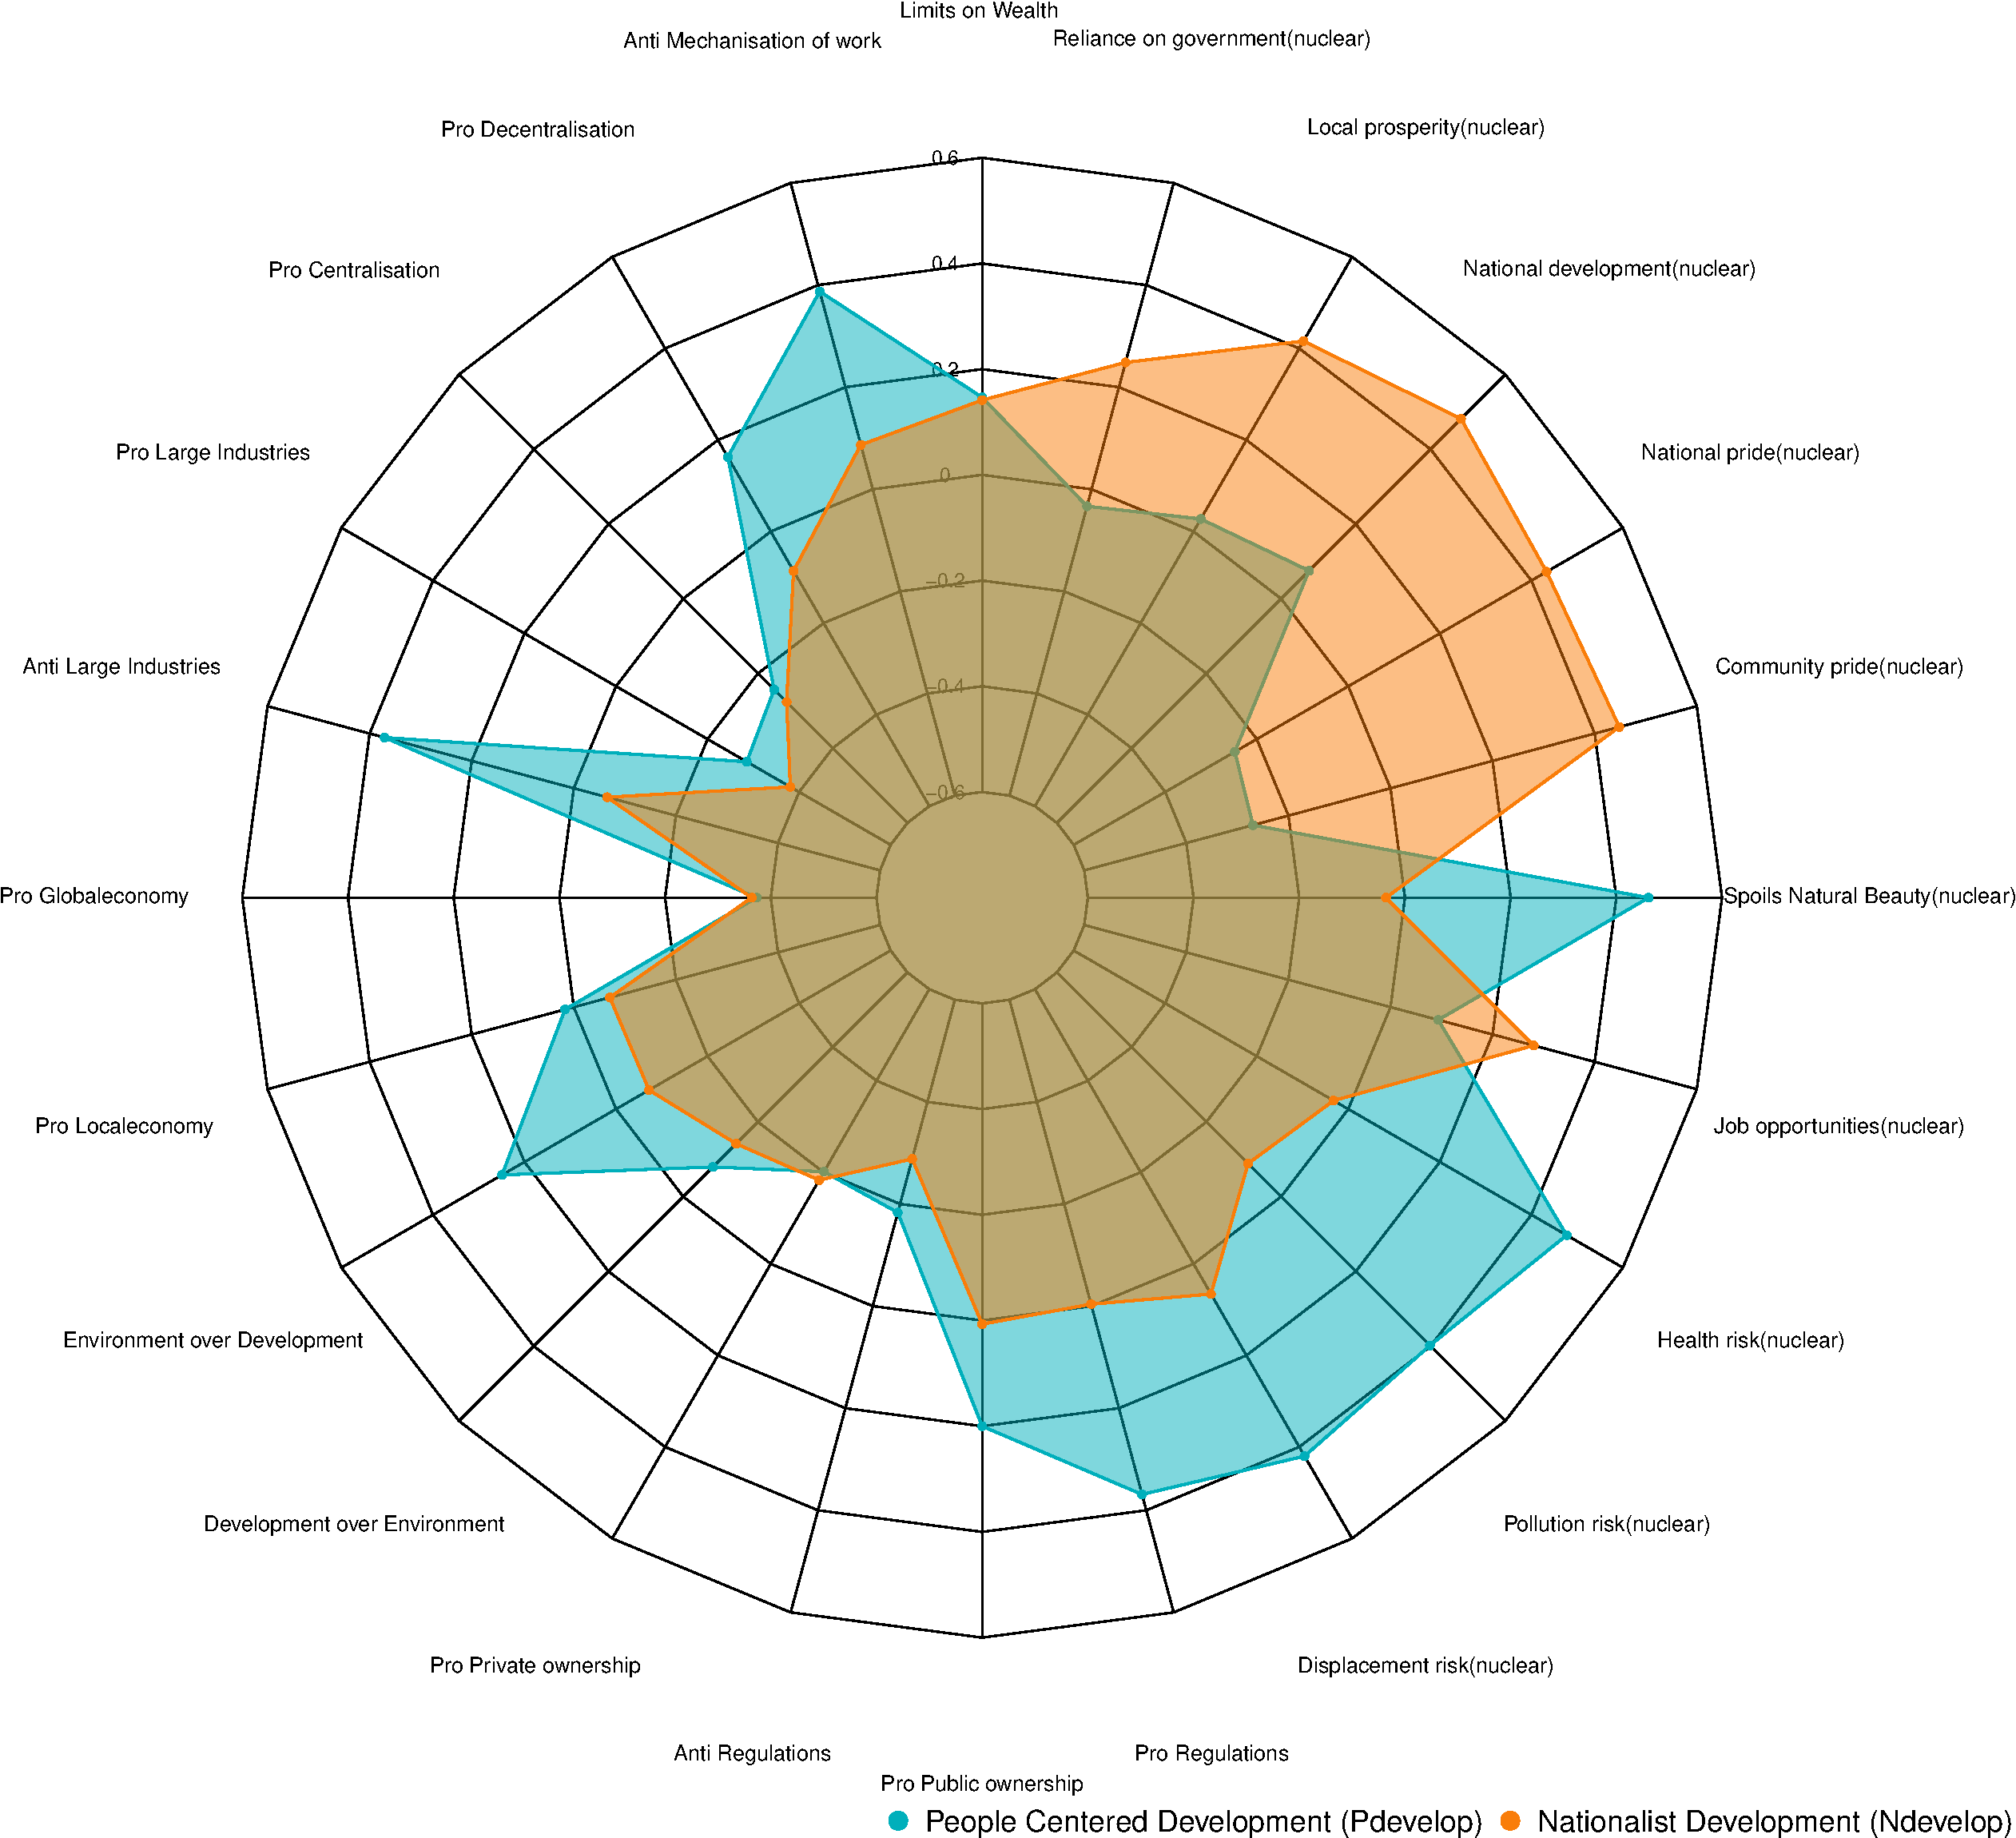
\includegraphics[width=1\linewidth,height=1\textheight]{corstuff_files/figure-latex/unnamed-chunk-18-1}

\newpage

\global\setlength{\Oldarrayrulewidth}{\arrayrulewidth}

\global\setlength{\Oldtabcolsep}{\tabcolsep}

\setlength{\tabcolsep}{0pt}

\renewcommand*{\arraystretch}{1.5}



\providecommand{\ascline}[3]{\noalign{\global\arrayrulewidth #1}\arrayrulecolor[HTML]{#2}\cline{#3}}

\begin{longtable}[c]{cccccc}

\caption{Eco-Pol\ Values\ Factor\ Analysis\ Table}\\

\ascline{1.5pt}{666666}{1-6}

\multicolumn{1}{>{}l}{\textcolor[HTML]{000000}{\fontsize{10}{10}\selectfont{Items}}} & \multicolumn{1}{>{}r}{\textcolor[HTML]{000000}{\fontsize{10}{10}\selectfont{Pdevelop}}} & \multicolumn{1}{>{}r}{\textcolor[HTML]{000000}{\fontsize{10}{10}\selectfont{Ndevelop}}} & \multicolumn{1}{>{}r}{\textcolor[HTML]{000000}{\fontsize{10}{10}\selectfont{Communality}}} & \multicolumn{1}{>{}r}{\textcolor[HTML]{000000}{\fontsize{10}{10}\selectfont{Uniqueness}}} & \multicolumn{1}{>{}r}{\textcolor[HTML]{000000}{\fontsize{10}{10}\selectfont{Complexity}}} \\

\ascline{1.5pt}{666666}{1-6}\endfirsthead \caption[]{Eco-Pol\ Values\ Factor\ Analysis\ Table}\\

\ascline{1.5pt}{666666}{1-6}

\multicolumn{1}{>{}l}{\textcolor[HTML]{000000}{\fontsize{10}{10}\selectfont{Items}}} & \multicolumn{1}{>{}r}{\textcolor[HTML]{000000}{\fontsize{10}{10}\selectfont{Pdevelop}}} & \multicolumn{1}{>{}r}{\textcolor[HTML]{000000}{\fontsize{10}{10}\selectfont{Ndevelop}}} & \multicolumn{1}{>{}r}{\textcolor[HTML]{000000}{\fontsize{10}{10}\selectfont{Communality}}} & \multicolumn{1}{>{}r}{\textcolor[HTML]{000000}{\fontsize{10}{10}\selectfont{Uniqueness}}} & \multicolumn{1}{>{}r}{\textcolor[HTML]{000000}{\fontsize{10}{10}\selectfont{Complexity}}} \\

\ascline{1.5pt}{666666}{1-6}\endhead



\multicolumn{1}{>{}l}{\textcolor[HTML]{000000}{\fontsize{10}{10}\selectfont{Health\ risk(nuclear)}}} & \multicolumn{1}{>{}r}{\textcolor[HTML]{000000}{\fontsize{10}{10}\selectfont{0.657}}} & \multicolumn{1}{>{}r}{\textcolor[HTML]{000000}{\fontsize{10}{10}\selectfont{0.062}}} & \multicolumn{1}{>{}r}{\textcolor[HTML]{000000}{\fontsize{10}{10}\selectfont{0.435}}} & \multicolumn{1}{>{}r}{\textcolor[HTML]{000000}{\fontsize{10}{10}\selectfont{0.565}}} & \multicolumn{1}{>{}r}{\textcolor[HTML]{000000}{\fontsize{10}{10}\selectfont{1.018}}} \\





\multicolumn{1}{>{}l}{\textcolor[HTML]{000000}{\fontsize{10}{10}\selectfont{Spoils\ Natural\ Beauty(nuclear)}}} & \multicolumn{1}{>{}r}{\textcolor[HTML]{000000}{\fontsize{10}{10}\selectfont{0.638}}} & \multicolumn{1}{>{}r}{\textcolor[HTML]{000000}{\fontsize{10}{10}\selectfont{0.058}}} & \multicolumn{1}{>{}r}{\textcolor[HTML]{000000}{\fontsize{10}{10}\selectfont{0.410}}} & \multicolumn{1}{>{}r}{\textcolor[HTML]{000000}{\fontsize{10}{10}\selectfont{0.590}}} & \multicolumn{1}{>{}r}{\textcolor[HTML]{000000}{\fontsize{10}{10}\selectfont{1.017}}} \\





\multicolumn{1}{>{}l}{\textcolor[HTML]{000000}{\fontsize{10}{10}\selectfont{Displacement\ risk(nuclear)}}} & \multicolumn{1}{>{}r}{\textcolor[HTML]{000000}{\fontsize{10}{10}\selectfont{0.590}}} & \multicolumn{1}{>{}r}{\textcolor[HTML]{000000}{\fontsize{10}{10}\selectfont{0.177}}} & \multicolumn{1}{>{}r}{\textcolor[HTML]{000000}{\fontsize{10}{10}\selectfont{0.380}}} & \multicolumn{1}{>{}r}{\textcolor[HTML]{000000}{\fontsize{10}{10}\selectfont{0.620}}} & \multicolumn{1}{>{}r}{\textcolor[HTML]{000000}{\fontsize{10}{10}\selectfont{1.178}}} \\





\multicolumn{1}{>{}l}{\textcolor[HTML]{000000}{\fontsize{10}{10}\selectfont{Pollution\ risk(nuclear)}}} & \multicolumn{1}{>{}r}{\textcolor[HTML]{000000}{\fontsize{10}{10}\selectfont{0.565}}} & \multicolumn{1}{>{}r}{\textcolor[HTML]{000000}{\fontsize{10}{10}\selectfont{-0.003}}} & \multicolumn{1}{>{}r}{\textcolor[HTML]{000000}{\fontsize{10}{10}\selectfont{0.319}}} & \multicolumn{1}{>{}r}{\textcolor[HTML]{000000}{\fontsize{10}{10}\selectfont{0.681}}} & \multicolumn{1}{>{}r}{\textcolor[HTML]{000000}{\fontsize{10}{10}\selectfont{1.000}}} \\





\multicolumn{1}{>{}l}{\textcolor[HTML]{000000}{\fontsize{10}{10}\selectfont{Anti\ Mechanisation\ of\ work}}} & \multicolumn{1}{>{}r}{\textcolor[HTML]{000000}{\fontsize{10}{10}\selectfont{0.552}}} & \multicolumn{1}{>{}r}{\textcolor[HTML]{000000}{\fontsize{10}{10}\selectfont{0.201}}} & \multicolumn{1}{>{}r}{\textcolor[HTML]{000000}{\fontsize{10}{10}\selectfont{0.345}}} & \multicolumn{1}{>{}r}{\textcolor[HTML]{000000}{\fontsize{10}{10}\selectfont{0.655}}} & \multicolumn{1}{>{}r}{\textcolor[HTML]{000000}{\fontsize{10}{10}\selectfont{1.262}}} \\





\multicolumn{1}{>{}l}{\textcolor[HTML]{000000}{\fontsize{10}{10}\selectfont{Anti\ Large\ Industries}}} & \multicolumn{1}{>{}r}{\textcolor[HTML]{000000}{\fontsize{10}{10}\selectfont{0.532}}} & \multicolumn{1}{>{}r}{\textcolor[HTML]{000000}{\fontsize{10}{10}\selectfont{0.024}}} & \multicolumn{1}{>{}r}{\textcolor[HTML]{000000}{\fontsize{10}{10}\selectfont{0.284}}} & \multicolumn{1}{>{}r}{\textcolor[HTML]{000000}{\fontsize{10}{10}\selectfont{0.716}}} & \multicolumn{1}{>{}r}{\textcolor[HTML]{000000}{\fontsize{10}{10}\selectfont{1.004}}} \\





\multicolumn{1}{>{}l}{\textcolor[HTML]{000000}{\fontsize{10}{10}\selectfont{Pro\ Regulations}}} & \multicolumn{1}{>{}r}{\textcolor[HTML]{000000}{\fontsize{10}{10}\selectfont{0.530}}} & \multicolumn{1}{>{}r}{\textcolor[HTML]{000000}{\fontsize{10}{10}\selectfont{0.096}}} & \multicolumn{1}{>{}r}{\textcolor[HTML]{000000}{\fontsize{10}{10}\selectfont{0.290}}} & \multicolumn{1}{>{}r}{\textcolor[HTML]{000000}{\fontsize{10}{10}\selectfont{0.710}}} & \multicolumn{1}{>{}r}{\textcolor[HTML]{000000}{\fontsize{10}{10}\selectfont{1.065}}} \\





\multicolumn{1}{>{}l}{\textcolor[HTML]{000000}{\fontsize{10}{10}\selectfont{Environment\ over\ Development}}} & \multicolumn{1}{>{}r}{\textcolor[HTML]{000000}{\fontsize{10}{10}\selectfont{0.391}}} & \multicolumn{1}{>{}r}{\textcolor[HTML]{000000}{\fontsize{10}{10}\selectfont{0.016}}} & \multicolumn{1}{>{}r}{\textcolor[HTML]{000000}{\fontsize{10}{10}\selectfont{0.153}}} & \multicolumn{1}{>{}r}{\textcolor[HTML]{000000}{\fontsize{10}{10}\selectfont{0.847}}} & \multicolumn{1}{>{}r}{\textcolor[HTML]{000000}{\fontsize{10}{10}\selectfont{1.003}}} \\





\multicolumn{1}{>{}l}{\textcolor[HTML]{000000}{\fontsize{10}{10}\selectfont{Pro\ Globaleconomy}}} & \multicolumn{1}{>{}r}{\textcolor[HTML]{000000}{\fontsize{10}{10}\selectfont{-0.335}}} & \multicolumn{1}{>{}r}{\textcolor[HTML]{000000}{\fontsize{10}{10}\selectfont{-0.325}}} & \multicolumn{1}{>{}r}{\textcolor[HTML]{000000}{\fontsize{10}{10}\selectfont{0.218}}} & \multicolumn{1}{>{}r}{\textcolor[HTML]{000000}{\fontsize{10}{10}\selectfont{0.782}}} & \multicolumn{1}{>{}r}{\textcolor[HTML]{000000}{\fontsize{10}{10}\selectfont{1.998}}} \\





\multicolumn{1}{>{}l}{\textcolor[HTML]{000000}{\fontsize{10}{10}\selectfont{Pro\ Public\ ownership}}} & \multicolumn{1}{>{}r}{\textcolor[HTML]{000000}{\fontsize{10}{10}\selectfont{0.333}}} & \multicolumn{1}{>{}r}{\textcolor[HTML]{000000}{\fontsize{10}{10}\selectfont{0.108}}} & \multicolumn{1}{>{}r}{\textcolor[HTML]{000000}{\fontsize{10}{10}\selectfont{0.123}}} & \multicolumn{1}{>{}r}{\textcolor[HTML]{000000}{\fontsize{10}{10}\selectfont{0.877}}} & \multicolumn{1}{>{}r}{\textcolor[HTML]{000000}{\fontsize{10}{10}\selectfont{1.208}}} \\





\multicolumn{1}{>{}l}{\textcolor[HTML]{000000}{\fontsize{10}{10}\selectfont{Pro\ Decentralisation}}} & \multicolumn{1}{>{}r}{\textcolor[HTML]{000000}{\fontsize{10}{10}\selectfont{0.290}}} & \multicolumn{1}{>{}r}{\textcolor[HTML]{000000}{\fontsize{10}{10}\selectfont{-0.001}}} & \multicolumn{1}{>{}r}{\textcolor[HTML]{000000}{\fontsize{10}{10}\selectfont{0.084}}} & \multicolumn{1}{>{}r}{\textcolor[HTML]{000000}{\fontsize{10}{10}\selectfont{0.916}}} & \multicolumn{1}{>{}r}{\textcolor[HTML]{000000}{\fontsize{10}{10}\selectfont{1.000}}} \\





\multicolumn{1}{>{}l}{\textcolor[HTML]{000000}{\fontsize{10}{10}\selectfont{Limits\ on\ Wealth}}} & \multicolumn{1}{>{}r}{\textcolor[HTML]{000000}{\fontsize{10}{10}\selectfont{0.271}}} & \multicolumn{1}{>{}r}{\textcolor[HTML]{000000}{\fontsize{10}{10}\selectfont{0.265}}} & \multicolumn{1}{>{}r}{\textcolor[HTML]{000000}{\fontsize{10}{10}\selectfont{0.144}}} & \multicolumn{1}{>{}r}{\textcolor[HTML]{000000}{\fontsize{10}{10}\selectfont{0.856}}} & \multicolumn{1}{>{}r}{\textcolor[HTML]{000000}{\fontsize{10}{10}\selectfont{1.999}}} \\





\multicolumn{1}{>{}l}{\textcolor[HTML]{000000}{\fontsize{10}{10}\selectfont{Pro\ Private\ ownership}}} & \multicolumn{1}{>{}r}{\textcolor[HTML]{000000}{\fontsize{10}{10}\selectfont{-0.135}}} & \multicolumn{1}{>{}r}{\textcolor[HTML]{000000}{\fontsize{10}{10}\selectfont{-0.113}}} & \multicolumn{1}{>{}r}{\textcolor[HTML]{000000}{\fontsize{10}{10}\selectfont{0.031}}} & \multicolumn{1}{>{}r}{\textcolor[HTML]{000000}{\fontsize{10}{10}\selectfont{0.969}}} & \multicolumn{1}{>{}r}{\textcolor[HTML]{000000}{\fontsize{10}{10}\selectfont{1.943}}} \\





\multicolumn{1}{>{}l}{\textcolor[HTML]{000000}{\fontsize{10}{10}\selectfont{Pro\ Localeconomy}}} & \multicolumn{1}{>{}r}{\textcolor[HTML]{000000}{\fontsize{10}{10}\selectfont{0.120}}} & \multicolumn{1}{>{}r}{\textcolor[HTML]{000000}{\fontsize{10}{10}\selectfont{0.018}}} & \multicolumn{1}{>{}r}{\textcolor[HTML]{000000}{\fontsize{10}{10}\selectfont{0.015}}} & \multicolumn{1}{>{}r}{\textcolor[HTML]{000000}{\fontsize{10}{10}\selectfont{0.985}}} & \multicolumn{1}{>{}r}{\textcolor[HTML]{000000}{\fontsize{10}{10}\selectfont{1.043}}} \\





\multicolumn{1}{>{}l}{\textcolor[HTML]{000000}{\fontsize{10}{10}\selectfont{National\ development(nuclear)}}} & \multicolumn{1}{>{}r}{\textcolor[HTML]{000000}{\fontsize{10}{10}\selectfont{0.187}}} & \multicolumn{1}{>{}r}{\textcolor[HTML]{000000}{\fontsize{10}{10}\selectfont{0.662}}} & \multicolumn{1}{>{}r}{\textcolor[HTML]{000000}{\fontsize{10}{10}\selectfont{0.473}}} & \multicolumn{1}{>{}r}{\textcolor[HTML]{000000}{\fontsize{10}{10}\selectfont{0.527}}} & \multicolumn{1}{>{}r}{\textcolor[HTML]{000000}{\fontsize{10}{10}\selectfont{1.159}}} \\





\multicolumn{1}{>{}l}{\textcolor[HTML]{000000}{\fontsize{10}{10}\selectfont{Community\ pride(nuclear)}}} & \multicolumn{1}{>{}r}{\textcolor[HTML]{000000}{\fontsize{10}{10}\selectfont{-0.215}}} & \multicolumn{1}{>{}r}{\textcolor[HTML]{000000}{\fontsize{10}{10}\selectfont{0.623}}} & \multicolumn{1}{>{}r}{\textcolor[HTML]{000000}{\fontsize{10}{10}\selectfont{0.434}}} & \multicolumn{1}{>{}r}{\textcolor[HTML]{000000}{\fontsize{10}{10}\selectfont{0.566}}} & \multicolumn{1}{>{}r}{\textcolor[HTML]{000000}{\fontsize{10}{10}\selectfont{1.234}}} \\





\multicolumn{1}{>{}l}{\textcolor[HTML]{000000}{\fontsize{10}{10}\selectfont{National\ pride(nuclear)}}} & \multicolumn{1}{>{}r}{\textcolor[HTML]{000000}{\fontsize{10}{10}\selectfont{-0.189}}} & \multicolumn{1}{>{}r}{\textcolor[HTML]{000000}{\fontsize{10}{10}\selectfont{0.605}}} & \multicolumn{1}{>{}r}{\textcolor[HTML]{000000}{\fontsize{10}{10}\selectfont{0.402}}} & \multicolumn{1}{>{}r}{\textcolor[HTML]{000000}{\fontsize{10}{10}\selectfont{0.598}}} & \multicolumn{1}{>{}r}{\textcolor[HTML]{000000}{\fontsize{10}{10}\selectfont{1.193}}} \\





\multicolumn{1}{>{}l}{\textcolor[HTML]{000000}{\fontsize{10}{10}\selectfont{Local\ prosperity(nuclear)}}} & \multicolumn{1}{>{}r}{\textcolor[HTML]{000000}{\fontsize{10}{10}\selectfont{0.132}}} & \multicolumn{1}{>{}r}{\textcolor[HTML]{000000}{\fontsize{10}{10}\selectfont{0.586}}} & \multicolumn{1}{>{}r}{\textcolor[HTML]{000000}{\fontsize{10}{10}\selectfont{0.360}}} & \multicolumn{1}{>{}r}{\textcolor[HTML]{000000}{\fontsize{10}{10}\selectfont{0.640}}} & \multicolumn{1}{>{}r}{\textcolor[HTML]{000000}{\fontsize{10}{10}\selectfont{1.101}}} \\





\multicolumn{1}{>{}l}{\textcolor[HTML]{000000}{\fontsize{10}{10}\selectfont{Job\ opportunities(nuclear)}}} & \multicolumn{1}{>{}r}{\textcolor[HTML]{000000}{\fontsize{10}{10}\selectfont{0.209}}} & \multicolumn{1}{>{}r}{\textcolor[HTML]{000000}{\fontsize{10}{10}\selectfont{0.427}}} & \multicolumn{1}{>{}r}{\textcolor[HTML]{000000}{\fontsize{10}{10}\selectfont{0.226}}} & \multicolumn{1}{>{}r}{\textcolor[HTML]{000000}{\fontsize{10}{10}\selectfont{0.774}}} & \multicolumn{1}{>{}r}{\textcolor[HTML]{000000}{\fontsize{10}{10}\selectfont{1.453}}} \\





\multicolumn{1}{>{}l}{\textcolor[HTML]{000000}{\fontsize{10}{10}\selectfont{Reliance\ on\ government(nuclear)}}} & \multicolumn{1}{>{}r}{\textcolor[HTML]{000000}{\fontsize{10}{10}\selectfont{0.061}}} & \multicolumn{1}{>{}r}{\textcolor[HTML]{000000}{\fontsize{10}{10}\selectfont{0.390}}} & \multicolumn{1}{>{}r}{\textcolor[HTML]{000000}{\fontsize{10}{10}\selectfont{0.156}}} & \multicolumn{1}{>{}r}{\textcolor[HTML]{000000}{\fontsize{10}{10}\selectfont{0.844}}} & \multicolumn{1}{>{}r}{\textcolor[HTML]{000000}{\fontsize{10}{10}\selectfont{1.049}}} \\





\multicolumn{1}{>{}l}{\textcolor[HTML]{000000}{\fontsize{10}{10}\selectfont{Pro\ Large\ Industries}}} & \multicolumn{1}{>{}r}{\textcolor[HTML]{000000}{\fontsize{10}{10}\selectfont{-0.233}}} & \multicolumn{1}{>{}r}{\textcolor[HTML]{000000}{\fontsize{10}{10}\selectfont{-0.344}}} & \multicolumn{1}{>{}r}{\textcolor[HTML]{000000}{\fontsize{10}{10}\selectfont{0.173}}} & \multicolumn{1}{>{}r}{\textcolor[HTML]{000000}{\fontsize{10}{10}\selectfont{0.827}}} & \multicolumn{1}{>{}r}{\textcolor[HTML]{000000}{\fontsize{10}{10}\selectfont{1.758}}} \\





\multicolumn{1}{>{}l}{\textcolor[HTML]{000000}{\fontsize{10}{10}\selectfont{Anti\ Regulations}}} & \multicolumn{1}{>{}r}{\textcolor[HTML]{000000}{\fontsize{10}{10}\selectfont{-0.114}}} & \multicolumn{1}{>{}r}{\textcolor[HTML]{000000}{\fontsize{10}{10}\selectfont{-0.236}}} & \multicolumn{1}{>{}r}{\textcolor[HTML]{000000}{\fontsize{10}{10}\selectfont{0.069}}} & \multicolumn{1}{>{}r}{\textcolor[HTML]{000000}{\fontsize{10}{10}\selectfont{0.931}}} & \multicolumn{1}{>{}r}{\textcolor[HTML]{000000}{\fontsize{10}{10}\selectfont{1.440}}} \\





\multicolumn{1}{>{}l}{\textcolor[HTML]{000000}{\fontsize{10}{10}\selectfont{Pro\ Centralisation}}} & \multicolumn{1}{>{}r}{\textcolor[HTML]{000000}{\fontsize{10}{10}\selectfont{-0.184}}} & \multicolumn{1}{>{}r}{\textcolor[HTML]{000000}{\fontsize{10}{10}\selectfont{-0.223}}} & \multicolumn{1}{>{}r}{\textcolor[HTML]{000000}{\fontsize{10}{10}\selectfont{0.083}}} & \multicolumn{1}{>{}r}{\textcolor[HTML]{000000}{\fontsize{10}{10}\selectfont{0.917}}} & \multicolumn{1}{>{}r}{\textcolor[HTML]{000000}{\fontsize{10}{10}\selectfont{1.930}}} \\





\multicolumn{1}{>{}l}{\textcolor[HTML]{000000}{\fontsize{10}{10}\selectfont{Development\ over\ Environment}}} & \multicolumn{1}{>{}r}{\textcolor[HTML]{000000}{\fontsize{10}{10}\selectfont{0.007}}} & \multicolumn{1}{>{}r}{\textcolor[HTML]{000000}{\fontsize{10}{10}\selectfont{-0.065}}} & \multicolumn{1}{>{}r}{\textcolor[HTML]{000000}{\fontsize{10}{10}\selectfont{0.004}}} & \multicolumn{1}{>{}r}{\textcolor[HTML]{000000}{\fontsize{10}{10}\selectfont{0.996}}} & \multicolumn{1}{>{}r}{\textcolor[HTML]{000000}{\fontsize{10}{10}\selectfont{1.025}}} \\

\ascline{1.5pt}{666666}{1-6}



\end{longtable}



\arrayrulecolor[HTML]{000000}

\global\setlength{\arrayrulewidth}{\Oldarrayrulewidth}

\global\setlength{\tabcolsep}{\Oldtabcolsep}

\renewcommand*{\arraystretch}{1}

\global\setlength{\Oldarrayrulewidth}{\arrayrulewidth}

\global\setlength{\Oldtabcolsep}{\tabcolsep}

\setlength{\tabcolsep}{0pt}

\renewcommand*{\arraystretch}{1.5}



\providecommand{\ascline}[3]{\noalign{\global\arrayrulewidth #1}\arrayrulecolor[HTML]{#2}\cline{#3}}

\begin{longtable}[c]{ccc}

\caption{Eigenvalues\ and\ Variance\ Explained\ for\ Rotated\ Factor\ Solution}\\

\ascline{1.5pt}{666666}{1-3}

\multicolumn{1}{>{}l}{\textcolor[HTML]{000000}{\fontsize{10}{10}\selectfont{Property}}} & \multicolumn{1}{>{}r}{\textcolor[HTML]{000000}{\fontsize{10}{10}\selectfont{Pdevelop}}} & \multicolumn{1}{>{}r}{\textcolor[HTML]{000000}{\fontsize{10}{10}\selectfont{Ndevelop}}} \\

\ascline{1.5pt}{666666}{1-3}\endfirsthead \caption[]{Eigenvalues\ and\ Variance\ Explained\ for\ Rotated\ Factor\ Solution}\\

\ascline{1.5pt}{666666}{1-3}

\multicolumn{1}{>{}l}{\textcolor[HTML]{000000}{\fontsize{10}{10}\selectfont{Property}}} & \multicolumn{1}{>{}r}{\textcolor[HTML]{000000}{\fontsize{10}{10}\selectfont{Pdevelop}}} & \multicolumn{1}{>{}r}{\textcolor[HTML]{000000}{\fontsize{10}{10}\selectfont{Ndevelop}}} \\

\ascline{1.5pt}{666666}{1-3}\endhead



\multicolumn{1}{>{}l}{\textcolor[HTML]{000000}{\fontsize{10}{10}\selectfont{SS\ loadings}}} & \multicolumn{1}{>{}r}{\textcolor[HTML]{000000}{\fontsize{10}{10}\selectfont{3.224}}} & \multicolumn{1}{>{}r}{\textcolor[HTML]{000000}{\fontsize{10}{10}\selectfont{2.388}}} \\





\multicolumn{1}{>{}l}{\textcolor[HTML]{000000}{\fontsize{10}{10}\selectfont{Proportion\ Var}}} & \multicolumn{1}{>{}r}{\textcolor[HTML]{000000}{\fontsize{10}{10}\selectfont{0.134}}} & \multicolumn{1}{>{}r}{\textcolor[HTML]{000000}{\fontsize{10}{10}\selectfont{0.099}}} \\





\multicolumn{1}{>{}l}{\textcolor[HTML]{000000}{\fontsize{10}{10}\selectfont{Cumulative\ Var}}} & \multicolumn{1}{>{}r}{\textcolor[HTML]{000000}{\fontsize{10}{10}\selectfont{0.134}}} & \multicolumn{1}{>{}r}{\textcolor[HTML]{000000}{\fontsize{10}{10}\selectfont{0.234}}} \\





\multicolumn{1}{>{}l}{\textcolor[HTML]{000000}{\fontsize{10}{10}\selectfont{Proportion\ Explained}}} & \multicolumn{1}{>{}r}{\textcolor[HTML]{000000}{\fontsize{10}{10}\selectfont{0.575}}} & \multicolumn{1}{>{}r}{\textcolor[HTML]{000000}{\fontsize{10}{10}\selectfont{0.425}}} \\





\multicolumn{1}{>{}l}{\textcolor[HTML]{000000}{\fontsize{10}{10}\selectfont{Cumulative\ Proportion}}} & \multicolumn{1}{>{}r}{\textcolor[HTML]{000000}{\fontsize{10}{10}\selectfont{0.575}}} & \multicolumn{1}{>{}r}{\textcolor[HTML]{000000}{\fontsize{10}{10}\selectfont{1.000}}} \\

\ascline{1.5pt}{666666}{1-3}



\end{longtable}



\arrayrulecolor[HTML]{000000}

\global\setlength{\arrayrulewidth}{\Oldarrayrulewidth}

\global\setlength{\tabcolsep}{\Oldtabcolsep}

\renewcommand*{\arraystretch}{1}

\newpage

\begin{landscape}
\begin{longtable}[t]{>{\raggedright\arraybackslash}p{4cm}>{\raggedright\arraybackslash}p{4cm}>{\raggedright\arraybackslash}p{9cm}ll}
\caption{\label{tab:unnamed-chunk-23}Two Factor Solution: Economic and Political Values Scale}\\
\toprule
Scale & Code & Items and Loadings & Alpha & Variance\\
\midrule
\endfirsthead
\caption[]{Two Factor Solution: Economic and Political Values Scale \textit{(continued)}}\\
\toprule
Scale & Code & Items and Loadings & Alpha & Variance\\
\midrule
\endhead

\endfoot
\bottomrule
\endlastfoot
\cellcolor{gray!6}{People Centered Development (Pdevelop)} & \cellcolor{gray!6}{Health risk(nuclear)} & \cellcolor{gray!6}{Nuclear energy poses a great risk to the health of people living around it.(0.657)} & \cellcolor{gray!6}{0.757} & \cellcolor{gray!6}{0.13}\\
 & Spoils Natural Beauty(nuclear) & Nuclear energy spoils the natural beauty of the landscape.(0.638) &  & \\
\cellcolor{gray!6}{} & \cellcolor{gray!6}{Anti Mechanisation of work} & \cellcolor{gray!6}{Rapid mechanization of work is taking away jobs from workers in this country.(0.552)} & \cellcolor{gray!6}{} & \cellcolor{gray!6}{}\\
 & Anti Large Industries & Large corporations are destroying the local industries in India and benefiting only a handful of people.(0.532) &  & \\
\cellcolor{gray!6}{} & \cellcolor{gray!6}{Displacement risk(nuclear)} & \cellcolor{gray!6}{Nuclear energy is leading to displacement of people from their land.(0.59)} & \cellcolor{gray!6}{} & \cellcolor{gray!6}{}\\
\addlinespace
 & Pollution risk(nuclear) & Nuclear energy increases pollution of air/water/land.(0.565) &  & \\
\cellcolor{gray!6}{} & \cellcolor{gray!6}{Pro Regulations} & \cellcolor{gray!6}{Regardless of ownership, the government should pass strong regulations and implement them.(0.53)} & \cellcolor{gray!6}{} & \cellcolor{gray!6}{}\\
Nationalist Development (Ndevelop) & National development(nuclear) & Nuclear energy pushes forward the country's development.(0.662) & 0.725 & 0.1\\
\cellcolor{gray!6}{} & \cellcolor{gray!6}{Community pride(nuclear)} & \cellcolor{gray!6}{I would be proud if my community used nuclear energy.(0.623)} & \cellcolor{gray!6}{} & \cellcolor{gray!6}{}\\
 & National pride(nuclear) & Nuclear energy is a mark of pride for our nation.(0.605) &  & \\
\addlinespace
\cellcolor{gray!6}{} & \cellcolor{gray!6}{Local prosperity(nuclear)} & \cellcolor{gray!6}{Nuclear energy brings economic prosperity to the surrounding regions.(0.586)} & \cellcolor{gray!6}{} & \cellcolor{gray!6}{}\\*
\end{longtable}
\end{landscape}

\newpage

\#Correlation table Eco-pol scale and Kahan CFA scores

\begin{verbatim}
##              KahanS     KahanH      Pdevelop      Ndevelop
## KahanS    1.0000000 -0.8446378 -6.481884e-01 -2.531260e-01
## KahanH   -0.8446378  1.0000000  6.300022e-01  3.078505e-01
## Pdevelop -0.6481884  0.6300022  1.000000e+00  1.746811e-15
## Ndevelop -0.2531260  0.3078505  1.746811e-15  1.000000e+00
\end{verbatim}

\hypertarget{correlation-eco-pol-and-alt-kahan-mean-across}{%
\section{Correlation Eco-pol and alt Kahan (mean
across)}\label{correlation-eco-pol-and-alt-kahan-mean-across}}

\begin{verbatim}
##                     Individualism_score Hierarchy_score      Pdevelop
## Individualism_score           1.0000000      0.39847778 -5.811795e-01
## Hierarchy_score               0.3984778      1.00000000 -5.252558e-01
## Pdevelop                     -0.5811795     -0.52525577  1.000000e+00
## Ndevelop                     -0.1627389     -0.08836034  1.746811e-15
##                          Ndevelop
## Individualism_score -1.627389e-01
## Hierarchy_score     -8.836034e-02
## Pdevelop             1.746811e-15
## Ndevelop             1.000000e+00
\end{verbatim}

\newpage

\hypertarget{scatter-plot-1-mean-across-kahan-scale-scores-around-medians}{%
\section{Scatter plot 1: mean across Kahan scale scores around
medians}\label{scatter-plot-1-mean-across-kahan-scale-scores-around-medians}}

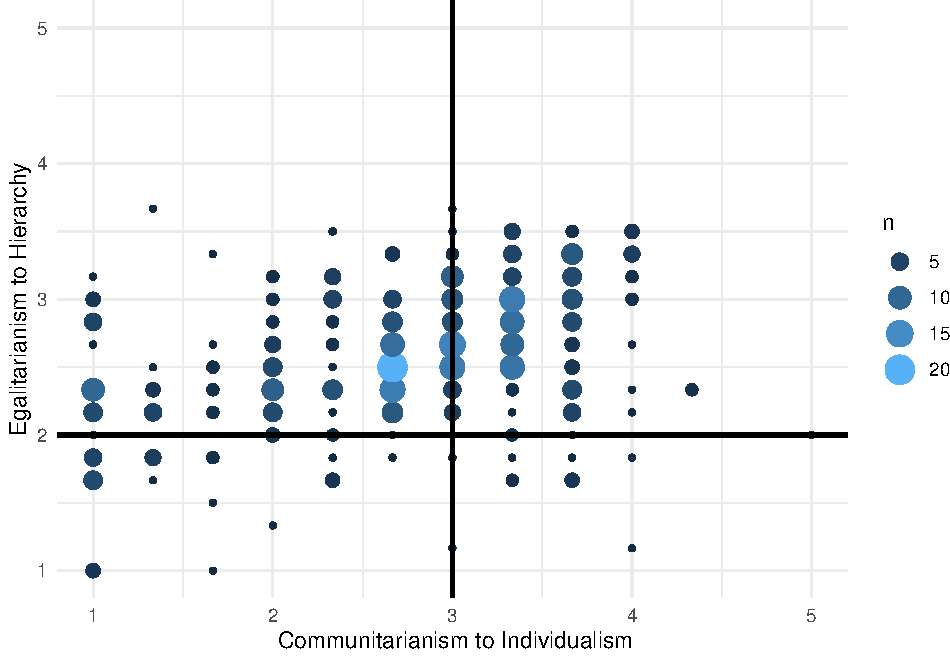
\includegraphics{corstuff_files/figure-latex/unnamed-chunk-27-1.pdf}

\hypertarget{scater-plot-2-kahan-cfa-scores}{%
\section{Scater plot 2: Kahan CFA
scores}\label{scater-plot-2-kahan-cfa-scores}}

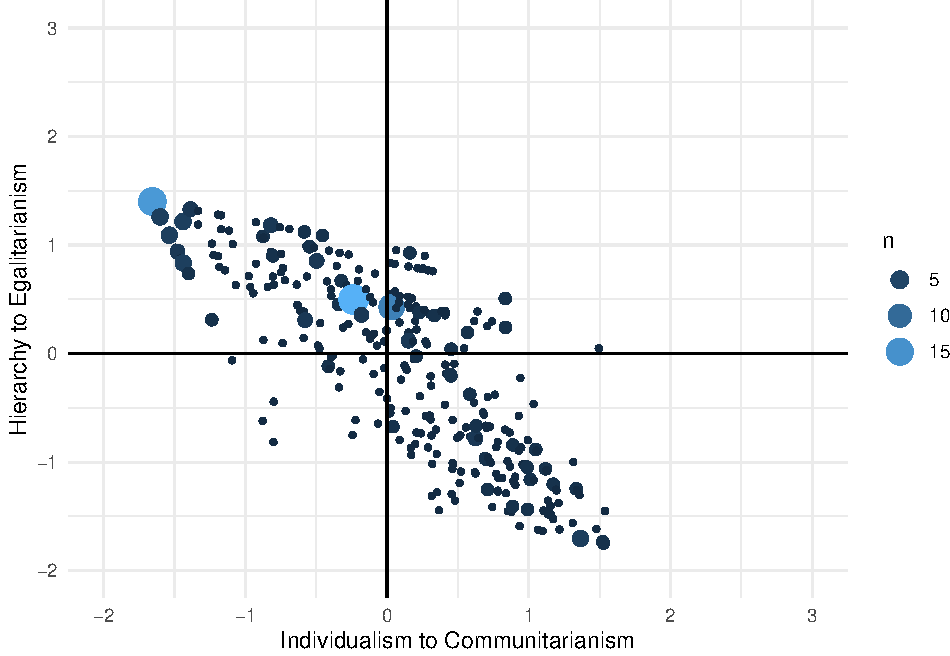
\includegraphics{corstuff_files/figure-latex/unnamed-chunk-28-1.pdf}

\newpage

\hypertarget{lms-with-alt-kahan-scores}{%
\section{Lms with alt Kahan scores}\label{lms-with-alt-kahan-scores}}

\begingroup\setlength{\tabcolsep}{1pt}

\renewcommand{\arraystretch}{0.7}

\% Table created by stargazer v.5.2.3 by Marek Hlavac, Social Policy
Institute. E-mail: marek.hlavac at gmail.com \% Date and time: Thu, Feb
01, 2024 - 09:39:05

\begin{table}[!htbp] \centering 
  \caption{Alternative Kahan Scores(mean acorss fixed factors)} 
  \label{} 
\begin{tabular}{@{\extracolsep{5pt}}lccc} 
\\[-1.8ex]\hline 
\hline \\[-1.8ex] 
 & \multicolumn{3}{c}{\textit{Dependent variable:}} \\ 
\cline{2-4} 
\\[-1.8ex] & \multicolumn{3}{c}{Risky\_Nuclear} \\ 
\\[-1.8ex] & (1) & (2) & (3)\\ 
\hline \\[-1.8ex] 
 Uppercaste & $-$0.041 & $-$0.042 & $-$0.040 \\ 
  & (0.107) & (0.105) & (0.105) \\ 
  & & & \\ 
 Male & $-$0.111 & $-$0.084 & $-$0.093 \\ 
  & (0.118) & (0.115) & (0.116) \\ 
  & & & \\ 
 Hindu & $-$0.025 & 0.027 & 0.020 \\ 
  & (0.118) & (0.117) & (0.117) \\ 
  & & & \\ 
 UrbanUrban & $-$0.001 & 0.034 & 0.021 \\ 
  & (0.112) & (0.110) & (0.111) \\ 
  & & & \\ 
 age & 0.054 & 0.038 & 0.041 \\ 
  & (0.052) & (0.051) & (0.051) \\ 
  & & & \\ 
 StateRajasthan & 0.494$^{***}$ & 0.186 & 0.194 \\ 
  & (0.165) & (0.180) & (0.180) \\ 
  & & & \\ 
 StateTamil Nadu & 1.029$^{***}$ & 1.322$^{***}$ & 1.218$^{***}$ \\ 
  & (0.208) & (0.239) & (0.246) \\ 
  & & & \\ 
 StateUttar Pradesh & 0.006 & $-$0.011 & $-$0.060 \\ 
  & (0.192) & (0.189) & (0.192) \\ 
  & & & \\ 
 StateWest Bengal & 1.166$^{***}$ & 1.017$^{***}$ & 0.976$^{***}$ \\ 
  & (0.213) & (0.223) & (0.225) \\ 
  & & & \\ 
 Individualism\_score & $-$0.157$^{**}$ &  & $-$0.061 \\ 
  & (0.065) &  & (0.070) \\ 
  & & & \\ 
 Hierarchy\_score & $-$0.287$^{***}$ &  & $-$0.161 \\ 
  & (0.111) &  & (0.114) \\ 
  & & & \\ 
 Pdevelop &  & 0.207$^{***}$ & 0.151$^{**}$ \\ 
  &  & (0.064) & (0.073) \\ 
  & & & \\ 
 Ndevelop &  & 0.256$^{***}$ & 0.228$^{***}$ \\ 
  &  & (0.057) & (0.059) \\ 
  & & & \\ 
 Constant & 4.166$^{***}$ & 3.011$^{***}$ & 3.617$^{***}$ \\ 
  & (0.368) & (0.171) & (0.390) \\ 
  & & & \\ 
\hline \\[-1.8ex] 
Observations & 405 & 405 & 405 \\ 
R$^{2}$ & 0.260 & 0.287 & 0.292 \\ 
Adjusted R$^{2}$ & 0.240 & 0.267 & 0.269 \\ 
Residual Std. Error & 0.941 (df = 393) & 0.924 (df = 393) & 0.923 (df = 391) \\ 
F Statistic & 12.583$^{***}$ (df = 11; 393) & 14.356$^{***}$ (df = 11; 393) & 12.408$^{***}$ (df = 13; 391) \\ 
\hline 
\hline \\[-1.8ex] 
\textit{Note:}  & \multicolumn{3}{r}{$^{*}$p$<$0.1; $^{**}$p$<$0.05; $^{***}$p$<$0.01} \\ 
\end{tabular} 
\end{table} 
\endgroup

\newpage

\hypertarget{lms-eco-pol-and-kahan-scale}{%
\section{LMs : eco-pol and kahan
scale}\label{lms-eco-pol-and-kahan-scale}}

\begingroup\setlength{\tabcolsep}{1pt}

\renewcommand{\arraystretch}{0.7}

\% Table created by stargazer v.5.2.3 by Marek Hlavac, Social Policy
Institute. E-mail: marek.hlavac at gmail.com \% Date and time: Thu, Feb
01, 2024 - 09:39:05

\begin{table}[!htbp] \centering 
  \caption{Lms with CFA Kahan} 
  \label{} 
\begin{tabular}{@{\extracolsep{5pt}}lccc} 
\\[-1.8ex]\hline 
\hline \\[-1.8ex] 
 & \multicolumn{3}{c}{\textit{Dependent variable:}} \\ 
\cline{2-4} 
\\[-1.8ex] & \multicolumn{3}{c}{Risky\_Nuclear} \\ 
\\[-1.8ex] & (1) & (2) & (3)\\ 
\hline \\[-1.8ex] 
 Uppercaste & $-$0.029 & $-$0.042 & $-$0.035 \\ 
  & (0.107) & (0.105) & (0.105) \\ 
  & & & \\ 
 Male & $-$0.102 & $-$0.084 & $-$0.085 \\ 
  & (0.117) & (0.115) & (0.116) \\ 
  & & & \\ 
 Hindu & $-$0.025 & 0.027 & 0.025 \\ 
  & (0.118) & (0.117) & (0.117) \\ 
  & & & \\ 
 UrbanUrban & $-$0.003 & 0.034 & 0.021 \\ 
  & (0.112) & (0.110) & (0.111) \\ 
  & & & \\ 
 age & 0.050 & 0.038 & 0.036 \\ 
  & (0.052) & (0.051) & (0.051) \\ 
  & & & \\ 
 StateRajasthan & 0.445$^{***}$ & 0.186 & 0.186 \\ 
  & (0.169) & (0.180) & (0.181) \\ 
  & & & \\ 
 StateTamil Nadu & 1.141$^{***}$ & 1.322$^{***}$ & 1.282$^{***}$ \\ 
  & (0.197) & (0.239) & (0.240) \\ 
  & & & \\ 
 StateUttar Pradesh & $-$0.006 & $-$0.011 & $-$0.061 \\ 
  & (0.192) & (0.189) & (0.193) \\ 
  & & & \\ 
 StateWest Bengal & 1.120$^{***}$ & 1.017$^{***}$ & 0.965$^{***}$ \\ 
  & (0.216) & (0.223) & (0.226) \\ 
  & & & \\ 
 KahanS & $-$0.202$^{*}$ &  & $-$0.120 \\ 
  & (0.110) &  & (0.111) \\ 
  & & & \\ 
 KahanH & 0.077 &  & $-$0.012 \\ 
  & (0.102) &  & (0.102) \\ 
  & & & \\ 
 Pdevelop &  & 0.207$^{***}$ & 0.159$^{**}$ \\ 
  &  & (0.064) & (0.075) \\ 
  & & & \\ 
 Ndevelop &  & 0.256$^{***}$ & 0.230$^{***}$ \\ 
  &  & (0.057) & (0.061) \\ 
  & & & \\ 
 Constant & 3.008$^{***}$ & 3.011$^{***}$ & 3.033$^{***}$ \\ 
  & (0.173) & (0.171) & (0.172) \\ 
  & & & \\ 
\hline \\[-1.8ex] 
Observations & 405 & 405 & 405 \\ 
R$^{2}$ & 0.260 & 0.287 & 0.290 \\ 
Adjusted R$^{2}$ & 0.240 & 0.267 & 0.267 \\ 
Residual Std. Error & 0.941 (df = 393) & 0.924 (df = 393) & 0.924 (df = 391) \\ 
F Statistic & 12.573$^{***}$ (df = 11; 393) & 14.356$^{***}$ (df = 11; 393) & 12.298$^{***}$ (df = 13; 391) \\ 
\hline 
\hline \\[-1.8ex] 
\textit{Note:}  & \multicolumn{3}{r}{$^{*}$p$<$0.1; $^{**}$p$<$0.05; $^{***}$p$<$0.01} \\ 
\end{tabular} 
\end{table} 
\endgroup

\newpage

\begin{landscape}

\hypertarget{kahan-scale-efa}{%
\section{Kahan scale EFA}\label{kahan-scale-efa}}

\global\setlength{\Oldarrayrulewidth}{\arrayrulewidth}

\global\setlength{\Oldtabcolsep}{\tabcolsep}

\setlength{\tabcolsep}{0pt}

\renewcommand*{\arraystretch}{1.5}



\providecommand{\ascline}[3]{\noalign{\global\arrayrulewidth #1}\arrayrulecolor[HTML]{#2}\cline{#3}}

\begin{longtable}[c]{cccccc}

\caption{Kahan\ Exploratory\ Factor\ Analysis\ Table}\\

\ascline{1.5pt}{666666}{1-6}

\multicolumn{1}{>{}l}{\textcolor[HTML]{000000}{\fontsize{11}{11}\selectfont{item}}} & \multicolumn{1}{>{}r}{\textcolor[HTML]{000000}{\fontsize{11}{11}\selectfont{MR1}}} & \multicolumn{1}{>{}r}{\textcolor[HTML]{000000}{\fontsize{11}{11}\selectfont{MR2}}} & \multicolumn{1}{>{}r}{\textcolor[HTML]{000000}{\fontsize{11}{11}\selectfont{Communality}}} & \multicolumn{1}{>{}r}{\textcolor[HTML]{000000}{\fontsize{11}{11}\selectfont{Uniqueness}}} & \multicolumn{1}{>{}r}{\textcolor[HTML]{000000}{\fontsize{11}{11}\selectfont{Complexity}}} \\

\ascline{1.5pt}{666666}{1-6}\endfirsthead \caption[]{Kahan\ Exploratory\ Factor\ Analysis\ Table}\\

\ascline{1.5pt}{666666}{1-6}

\multicolumn{1}{>{}l}{\textcolor[HTML]{000000}{\fontsize{11}{11}\selectfont{item}}} & \multicolumn{1}{>{}r}{\textcolor[HTML]{000000}{\fontsize{11}{11}\selectfont{MR1}}} & \multicolumn{1}{>{}r}{\textcolor[HTML]{000000}{\fontsize{11}{11}\selectfont{MR2}}} & \multicolumn{1}{>{}r}{\textcolor[HTML]{000000}{\fontsize{11}{11}\selectfont{Communality}}} & \multicolumn{1}{>{}r}{\textcolor[HTML]{000000}{\fontsize{11}{11}\selectfont{Uniqueness}}} & \multicolumn{1}{>{}r}{\textcolor[HTML]{000000}{\fontsize{11}{11}\selectfont{Complexity}}} \\

\ascline{1.5pt}{666666}{1-6}\endhead



\multicolumn{1}{>{}l}{\textcolor[HTML]{000000}{\fontsize{11}{11}\selectfont{(E)We\ need\ to\ dramatically\ reduce\ inequalities\ between\ the\ rich\ and\ the\ poor.}}} & \multicolumn{1}{>{}r}{\textcolor[HTML]{000000}{\fontsize{11}{11}\selectfont{0.655}}} & \multicolumn{1}{>{}r}{\textcolor[HTML]{000000}{\fontsize{11}{11}\selectfont{-0.109}}} & \multicolumn{1}{>{}r}{\textcolor[HTML]{000000}{\fontsize{11}{11}\selectfont{0.441}}} & \multicolumn{1}{>{}r}{\textcolor[HTML]{000000}{\fontsize{11}{11}\selectfont{0.559}}} & \multicolumn{1}{>{}r}{\textcolor[HTML]{000000}{\fontsize{11}{11}\selectfont{1.055}}} \\





\multicolumn{1}{>{}l}{\textcolor[HTML]{000000}{\fontsize{11}{11}\selectfont{(E)We\ need\ to\ dramatically\ reduce\ inequalities\ between\ men\ and\ women.}}} & \multicolumn{1}{>{}r}{\textcolor[HTML]{000000}{\fontsize{11}{11}\selectfont{0.634}}} & \multicolumn{1}{>{}r}{\textcolor[HTML]{000000}{\fontsize{11}{11}\selectfont{0.025}}} & \multicolumn{1}{>{}r}{\textcolor[HTML]{000000}{\fontsize{11}{11}\selectfont{0.403}}} & \multicolumn{1}{>{}r}{\textcolor[HTML]{000000}{\fontsize{11}{11}\selectfont{0.597}}} & \multicolumn{1}{>{}r}{\textcolor[HTML]{000000}{\fontsize{11}{11}\selectfont{1.003}}} \\





\multicolumn{1}{>{}l}{\textcolor[HTML]{000000}{\fontsize{11}{11}\selectfont{(E)Our\ society\ would\ be\ better\ off\ if\ the\ distribution\ of\ wealth\ was\ more\ equal.}}} & \multicolumn{1}{>{}r}{\textcolor[HTML]{000000}{\fontsize{11}{11}\selectfont{0.616}}} & \multicolumn{1}{>{}r}{\textcolor[HTML]{000000}{\fontsize{11}{11}\selectfont{-0.033}}} & \multicolumn{1}{>{}r}{\textcolor[HTML]{000000}{\fontsize{11}{11}\selectfont{0.381}}} & \multicolumn{1}{>{}r}{\textcolor[HTML]{000000}{\fontsize{11}{11}\selectfont{0.619}}} & \multicolumn{1}{>{}r}{\textcolor[HTML]{000000}{\fontsize{11}{11}\selectfont{1.006}}} \\





\multicolumn{1}{>{}l}{\textcolor[HTML]{000000}{\fontsize{11}{11}\selectfont{(C)Sometimes\ the\ government\ needs\ to\ make\ laws\ that\ keep\ people\ from\ hurting\ themselves.}}} & \multicolumn{1}{>{}r}{\textcolor[HTML]{000000}{\fontsize{11}{11}\selectfont{0.595}}} & \multicolumn{1}{>{}r}{\textcolor[HTML]{000000}{\fontsize{11}{11}\selectfont{-0.011}}} & \multicolumn{1}{>{}r}{\textcolor[HTML]{000000}{\fontsize{11}{11}\selectfont{0.354}}} & \multicolumn{1}{>{}r}{\textcolor[HTML]{000000}{\fontsize{11}{11}\selectfont{0.646}}} & \multicolumn{1}{>{}r}{\textcolor[HTML]{000000}{\fontsize{11}{11}\selectfont{1.001}}} \\





\multicolumn{1}{>{}l}{\textcolor[HTML]{000000}{\fontsize{11}{11}\selectfont{(C)The\ government\ should\ put\ limits\ on\ the\ choices\ individuals\ can\ make\ so\ they\ don’t\ get\ in\ the\ way\ of\ what’s\ good\ for\ society.}}} & \multicolumn{1}{>{}r}{\textcolor[HTML]{000000}{\fontsize{11}{11}\selectfont{0.571}}} & \multicolumn{1}{>{}r}{\textcolor[HTML]{000000}{\fontsize{11}{11}\selectfont{-0.095}}} & \multicolumn{1}{>{}r}{\textcolor[HTML]{000000}{\fontsize{11}{11}\selectfont{0.335}}} & \multicolumn{1}{>{}r}{\textcolor[HTML]{000000}{\fontsize{11}{11}\selectfont{0.665}}} & \multicolumn{1}{>{}r}{\textcolor[HTML]{000000}{\fontsize{11}{11}\selectfont{1.056}}} \\





\multicolumn{1}{>{}l}{\textcolor[HTML]{000000}{\fontsize{11}{11}\selectfont{(H)We\ have\ gone\ too\ far\ in\ pushing\ equal\ rights\ in\ this\ country.}}} & \multicolumn{1}{>{}r}{\textcolor[HTML]{000000}{\fontsize{11}{11}\selectfont{-0.525}}} & \multicolumn{1}{>{}r}{\textcolor[HTML]{000000}{\fontsize{11}{11}\selectfont{0.120}}} & \multicolumn{1}{>{}r}{\textcolor[HTML]{000000}{\fontsize{11}{11}\selectfont{0.290}}} & \multicolumn{1}{>{}r}{\textcolor[HTML]{000000}{\fontsize{11}{11}\selectfont{0.710}}} & \multicolumn{1}{>{}r}{\textcolor[HTML]{000000}{\fontsize{11}{11}\selectfont{1.103}}} \\





\multicolumn{1}{>{}l}{\textcolor[HTML]{000000}{\fontsize{11}{11}\selectfont{(C)The\ government\ should\ do\ more\ to\ advance\ society’s\ goals,\ even\ if\ that\ means\ limiting\ the\ freedom\ and\ choices\ of\ individuals.}}} & \multicolumn{1}{>{}r}{\textcolor[HTML]{000000}{\fontsize{11}{11}\selectfont{0.446}}} & \multicolumn{1}{>{}r}{\textcolor[HTML]{000000}{\fontsize{11}{11}\selectfont{-0.087}}} & \multicolumn{1}{>{}r}{\textcolor[HTML]{000000}{\fontsize{11}{11}\selectfont{0.207}}} & \multicolumn{1}{>{}r}{\textcolor[HTML]{000000}{\fontsize{11}{11}\selectfont{0.793}}} & \multicolumn{1}{>{}r}{\textcolor[HTML]{000000}{\fontsize{11}{11}\selectfont{1.076}}} \\





\multicolumn{1}{>{}l}{\textcolor[HTML]{000000}{\fontsize{11}{11}\selectfont{(I)The\ government\ interferes\ far\ too\ much\ in\ our\ everyday\ lives.}}} & \multicolumn{1}{>{}r}{\textcolor[HTML]{000000}{\fontsize{11}{11}\selectfont{-0.284}}} & \multicolumn{1}{>{}r}{\textcolor[HTML]{000000}{\fontsize{11}{11}\selectfont{0.128}}} & \multicolumn{1}{>{}r}{\textcolor[HTML]{000000}{\fontsize{11}{11}\selectfont{0.097}}} & \multicolumn{1}{>{}r}{\textcolor[HTML]{000000}{\fontsize{11}{11}\selectfont{0.903}}} & \multicolumn{1}{>{}r}{\textcolor[HTML]{000000}{\fontsize{11}{11}\selectfont{1.390}}} \\





\multicolumn{1}{>{}l}{\textcolor[HTML]{000000}{\fontsize{11}{11}\selectfont{(I)It’s\ not\ the\ government’s\ business\ to\ try\ to\ protect\ people\ from\ themselves.}}} & \multicolumn{1}{>{}r}{\textcolor[HTML]{000000}{\fontsize{11}{11}\selectfont{0.169}}} & \multicolumn{1}{>{}r}{\textcolor[HTML]{000000}{\fontsize{11}{11}\selectfont{0.110}}} & \multicolumn{1}{>{}r}{\textcolor[HTML]{000000}{\fontsize{11}{11}\selectfont{0.041}}} & \multicolumn{1}{>{}r}{\textcolor[HTML]{000000}{\fontsize{11}{11}\selectfont{0.959}}} & \multicolumn{1}{>{}r}{\textcolor[HTML]{000000}{\fontsize{11}{11}\selectfont{1.722}}} \\





\multicolumn{1}{>{}l}{\textcolor[HTML]{000000}{\fontsize{11}{11}\selectfont{(H)Nowadays\ it\ seems\ like\ there\ is\ just\ as\ much\ discrimination\ against\ upper\ castes\ as\ there\ is\ against\ Dalits.}}} & \multicolumn{1}{>{}r}{\textcolor[HTML]{000000}{\fontsize{11}{11}\selectfont{-0.147}}} & \multicolumn{1}{>{}r}{\textcolor[HTML]{000000}{\fontsize{11}{11}\selectfont{0.661}}} & \multicolumn{1}{>{}r}{\textcolor[HTML]{000000}{\fontsize{11}{11}\selectfont{0.459}}} & \multicolumn{1}{>{}r}{\textcolor[HTML]{000000}{\fontsize{11}{11}\selectfont{0.541}}} & \multicolumn{1}{>{}r}{\textcolor[HTML]{000000}{\fontsize{11}{11}\selectfont{1.099}}} \\





\multicolumn{1}{>{}l}{\textcolor[HTML]{000000}{\fontsize{11}{11}\selectfont{(E)Discrimination\ against\ minorities\ is\ still\ a\ very\ serious\ problem\ in\ our\ society.}}} & \multicolumn{1}{>{}r}{\textcolor[HTML]{000000}{\fontsize{11}{11}\selectfont{0.359}}} & \multicolumn{1}{>{}r}{\textcolor[HTML]{000000}{\fontsize{11}{11}\selectfont{-0.627}}} & \multicolumn{1}{>{}r}{\textcolor[HTML]{000000}{\fontsize{11}{11}\selectfont{0.522}}} & \multicolumn{1}{>{}r}{\textcolor[HTML]{000000}{\fontsize{11}{11}\selectfont{0.478}}} & \multicolumn{1}{>{}r}{\textcolor[HTML]{000000}{\fontsize{11}{11}\selectfont{1.593}}} \\





\multicolumn{1}{>{}l}{\textcolor[HTML]{000000}{\fontsize{11}{11}\selectfont{(I)The\ government\ should\ stop\ telling\ people\ how\ to\ live\ their\ lives.}}} & \multicolumn{1}{>{}r}{\textcolor[HTML]{000000}{\fontsize{11}{11}\selectfont{0.051}}} & \multicolumn{1}{>{}r}{\textcolor[HTML]{000000}{\fontsize{11}{11}\selectfont{0.291}}} & \multicolumn{1}{>{}r}{\textcolor[HTML]{000000}{\fontsize{11}{11}\selectfont{0.087}}} & \multicolumn{1}{>{}r}{\textcolor[HTML]{000000}{\fontsize{11}{11}\selectfont{0.913}}} & \multicolumn{1}{>{}r}{\textcolor[HTML]{000000}{\fontsize{11}{11}\selectfont{1.061}}} \\

\ascline{1.5pt}{666666}{1-6}



\end{longtable}



\arrayrulecolor[HTML]{000000}

\global\setlength{\arrayrulewidth}{\Oldarrayrulewidth}

\global\setlength{\tabcolsep}{\Oldtabcolsep}

\renewcommand*{\arraystretch}{1}

\end{landscape}

\newpage

\global\setlength{\Oldarrayrulewidth}{\arrayrulewidth}

\global\setlength{\Oldtabcolsep}{\tabcolsep}

\setlength{\tabcolsep}{0pt}

\renewcommand*{\arraystretch}{1.5}



\providecommand{\ascline}[3]{\noalign{\global\arrayrulewidth #1}\arrayrulecolor[HTML]{#2}\cline{#3}}

\begin{longtable}[c]{ccc}

\caption{Eigenvalues\ and\ Variance\ Explained\ for\ Rotated\ Factor\ Solution}\\

\ascline{1.5pt}{666666}{1-3}

\multicolumn{1}{>{}l}{\textcolor[HTML]{000000}{\fontsize{11}{11}\selectfont{Property}}} & \multicolumn{1}{>{}r}{\textcolor[HTML]{000000}{\fontsize{11}{11}\selectfont{MR1}}} & \multicolumn{1}{>{}r}{\textcolor[HTML]{000000}{\fontsize{11}{11}\selectfont{MR2}}} \\

\ascline{1.5pt}{666666}{1-3}\endfirsthead \caption[]{Eigenvalues\ and\ Variance\ Explained\ for\ Rotated\ Factor\ Solution}\\

\ascline{1.5pt}{666666}{1-3}

\multicolumn{1}{>{}l}{\textcolor[HTML]{000000}{\fontsize{11}{11}\selectfont{Property}}} & \multicolumn{1}{>{}r}{\textcolor[HTML]{000000}{\fontsize{11}{11}\selectfont{MR1}}} & \multicolumn{1}{>{}r}{\textcolor[HTML]{000000}{\fontsize{11}{11}\selectfont{MR2}}} \\

\ascline{1.5pt}{666666}{1-3}\endhead



\multicolumn{1}{>{}l}{\textcolor[HTML]{000000}{\fontsize{11}{11}\selectfont{SS\ loadings}}} & \multicolumn{1}{>{}r}{\textcolor[HTML]{000000}{\fontsize{11}{11}\selectfont{2.629}}} & \multicolumn{1}{>{}r}{\textcolor[HTML]{000000}{\fontsize{11}{11}\selectfont{0.988}}} \\





\multicolumn{1}{>{}l}{\textcolor[HTML]{000000}{\fontsize{11}{11}\selectfont{Proportion\ Var}}} & \multicolumn{1}{>{}r}{\textcolor[HTML]{000000}{\fontsize{11}{11}\selectfont{0.219}}} & \multicolumn{1}{>{}r}{\textcolor[HTML]{000000}{\fontsize{11}{11}\selectfont{0.082}}} \\





\multicolumn{1}{>{}l}{\textcolor[HTML]{000000}{\fontsize{11}{11}\selectfont{Cumulative\ Var}}} & \multicolumn{1}{>{}r}{\textcolor[HTML]{000000}{\fontsize{11}{11}\selectfont{0.219}}} & \multicolumn{1}{>{}r}{\textcolor[HTML]{000000}{\fontsize{11}{11}\selectfont{0.301}}} \\





\multicolumn{1}{>{}l}{\textcolor[HTML]{000000}{\fontsize{11}{11}\selectfont{Proportion\ Explained}}} & \multicolumn{1}{>{}r}{\textcolor[HTML]{000000}{\fontsize{11}{11}\selectfont{0.727}}} & \multicolumn{1}{>{}r}{\textcolor[HTML]{000000}{\fontsize{11}{11}\selectfont{0.273}}} \\





\multicolumn{1}{>{}l}{\textcolor[HTML]{000000}{\fontsize{11}{11}\selectfont{Cumulative\ Proportion}}} & \multicolumn{1}{>{}r}{\textcolor[HTML]{000000}{\fontsize{11}{11}\selectfont{0.727}}} & \multicolumn{1}{>{}r}{\textcolor[HTML]{000000}{\fontsize{11}{11}\selectfont{1.000}}} \\

\ascline{1.5pt}{666666}{1-3}



\end{longtable}



\arrayrulecolor[HTML]{000000}

\global\setlength{\arrayrulewidth}{\Oldarrayrulewidth}

\global\setlength{\tabcolsep}{\Oldtabcolsep}

\renewcommand*{\arraystretch}{1}

\newpage

\hypertarget{lms-with-efa-kahan-factors}{%
\section{LMs with EFA Kahan factors}\label{lms-with-efa-kahan-factors}}

\begingroup\setlength{\tabcolsep}{1pt}

\renewcommand{\arraystretch}{0.7}

\% Table created by stargazer v.5.2.3 by Marek Hlavac, Social Policy
Institute. E-mail: marek.hlavac at gmail.com \% Date and time: Thu, Feb
01, 2024 - 09:39:06

\begin{table}[!htbp] \centering 
  \caption{Lms with CFA Kahan} 
  \label{} 
\begin{tabular}{@{\extracolsep{5pt}}lccc} 
\\[-1.8ex]\hline 
\hline \\[-1.8ex] 
 & \multicolumn{3}{c}{\textit{Dependent variable:}} \\ 
\cline{2-4} 
\\[-1.8ex] & \multicolumn{3}{c}{Risky\_Nuclear} \\ 
\\[-1.8ex] & (1) & (2) & (3)\\ 
\hline \\[-1.8ex] 
 Uppercaste & 0.059 & $-$0.117 & $-$0.109 \\ 
  & (0.105) & (0.097) & (0.096) \\ 
  & & & \\ 
 Male & 0.081 & 0.011 & $-$0.010 \\ 
  & (0.105) & (0.105) & (0.105) \\ 
  & & & \\ 
 Hindu & $-$0.201$^{*}$ & $-$0.144 & $-$0.154 \\ 
  & (0.121) & (0.112) & (0.111) \\ 
  & & & \\ 
 UrbanUrban & $-$0.194$^{*}$ & 0.065 & 0.047 \\ 
  & (0.102) & (0.103) & (0.102) \\ 
  & & & \\ 
 age &  & $-$0.132$^{***}$ & $-$0.129$^{***}$ \\ 
  &  & (0.041) & (0.041) \\ 
  & & & \\ 
 StateRajasthan &  & 0.487$^{***}$ & 0.110 \\ 
  &  & (0.147) & (0.175) \\ 
  & & & \\ 
 StateTamil Nadu &  & 0.118 & $-$0.195 \\ 
  &  & (0.142) & (0.160) \\ 
  & & & \\ 
 StateUttar Pradesh &  & 0.146 & $-$0.061 \\ 
  &  & (0.167) & (0.172) \\ 
  & & & \\ 
 StateWest Bengal &  & 1.589$^{***}$ & 1.280$^{***}$ \\ 
  &  & (0.143) & (0.160) \\ 
  & & & \\ 
 CE &  &  & $-$0.209$^{***}$ \\ 
  &  &  & (0.054) \\ 
  & & & \\ 
 HE &  &  & $-$0.115$^{**}$ \\ 
  &  &  & (0.050) \\ 
  & & & \\ 
 Constant & 3.492$^{***}$ & 3.397$^{***}$ & 3.604$^{***}$ \\ 
  & (0.146) & (0.154) & (0.160) \\ 
  & & & \\ 
\hline \\[-1.8ex] 
Observations & 638 & 638 & 638 \\ 
R$^{2}$ & 0.012 & 0.202 & 0.223 \\ 
Adjusted R$^{2}$ & 0.006 & 0.190 & 0.209 \\ 
Residual Std. Error & 1.203 (df = 633) & 1.086 (df = 628) & 1.073 (df = 626) \\ 
F Statistic & 1.942 (df = 4; 633) & 17.609$^{***}$ (df = 9; 628) & 16.325$^{***}$ (df = 11; 626) \\ 
\hline 
\hline \\[-1.8ex] 
\textit{Note:}  & \multicolumn{3}{r}{$^{*}$p$<$0.1; $^{**}$p$<$0.05; $^{***}$p$<$0.01} \\ 
\end{tabular} 
\end{table} 
\endgroup

\newpage

\hypertarget{extra-kahan-scale-efa}{%
\section{2. EXTRA:: Kahan scale EFA}\label{extra-kahan-scale-efa}}

\begin{verbatim}
## Factor Analysis using method =  minres
## Call: fa(r = Kahan_scale2, nfactors = 2, rotate = "varimax")
## Standardized loadings (pattern matrix) based upon correlation matrix
##            item   MR1   MR2    h2   u2 com
## K_ERADEQ1    10  0.71       0.521 0.48 1.0
## K_ERADEQ2    12  0.70       0.503 0.50 1.0
## K_HEQUAL      7 -0.59       0.347 0.65 1.0
## K_SHARM       3  0.57       0.338 0.66 1.1
## K_EWEALTH    11  0.55       0.300 0.70 1.0
## K_SLIMCHOI    5  0.53       0.289 0.71 1.1
## K_IINTRFER    1 -0.41       0.177 0.82 1.2
## K_SPROTECT    6             0.153 0.85 1.1
## K_EDISCRIM    9  0.41 -0.53 0.452 0.55 1.9
## K_HREVDIS1    8        0.50 0.278 0.72 1.2
## K_IPROTECT    4             0.130 0.87 1.1
## K_IPRIVACY    2             0.071 0.93 1.0
## 
##                        MR1  MR2
## SS loadings           2.77 0.79
## Proportion Var        0.23 0.07
## Cumulative Var        0.23 0.30
## Proportion Explained  0.78 0.22
## Cumulative Proportion 0.78 1.00
## 
## Mean item complexity =  1.1
## Test of the hypothesis that 2 factors are sufficient.
## 
## df null model =  66  with the objective function =  2.56 with Chi Square =  1020.5
## df of  the model are 43  and the objective function was  0.55 
## 
## The root mean square of the residuals (RMSR) is  0.07 
## The df corrected root mean square of the residuals is  0.09 
## 
## The harmonic n.obs is  405 with the empirical chi square  255.04  with prob <  6.5e-32 
## The total n.obs was  405  with Likelihood Chi Square =  219.79  with prob <  1.4e-25 
## 
## Tucker Lewis Index of factoring reliability =  0.715
## RMSEA index =  0.101  and the 90 % confidence intervals are  0.088 0.114
## BIC =  -38.38
## Fit based upon off diagonal values = 0.92
## Measures of factor score adequacy             
##                                                    MR1  MR2
## Correlation of (regression) scores with factors   0.90 0.73
## Multiple R square of scores with factors          0.82 0.53
## Minimum correlation of possible factor scores     0.63 0.06
\end{verbatim}

\hypertarget{lms-with-efa-kahan-factors-1}{%
\section{2. LMs with EFA Kahan
factors}\label{lms-with-efa-kahan-factors-1}}

\newpage

\hypertarget{lms-by-state}{%
\section{LMs by State}\label{lms-by-state}}

\begin{verbatim}
## 
## Call:
## lm(formula = Risky_Nuclear ~ Uppercaste + Male + Hindu + Urban + 
##     age, data = TMalldemos)
## 
## Residuals:
##      Min       1Q   Median       3Q      Max 
## -2.78789 -0.86641 -0.03328  0.97482  2.32058 
## 
## Coefficients:
##             Estimate Std. Error t value Pr(>|t|)    
## (Intercept)  3.41615    0.36862   9.267  < 2e-16 ***
## Uppercaste  -0.33640    0.21743  -1.547  0.12310    
## Male         0.41820    0.15984   2.616  0.00943 ** 
## Hindu       -0.26214    0.34753  -0.754  0.45139    
## UrbanUrban   0.69026    0.17070   4.044 7.03e-05 ***
## age         -0.23729    0.05612  -4.229 3.31e-05 ***
## ---
## Signif. codes:  0 '***' 0.001 '**' 0.01 '*' 0.05 '.' 0.1 ' ' 1
## 
## Residual standard error: 1.209 on 248 degrees of freedom
##   (66 observations deleted due to missingness)
## Multiple R-squared:  0.1277, Adjusted R-squared:  0.1101 
## F-statistic: 7.263 on 5 and 248 DF,  p-value: 2.28e-06
\end{verbatim}

\begin{verbatim}
## 
## Call:
## lm(formula = Risky_Nuclear ~ Uppercaste + Male + Hindu + Urban + 
##     age + Pdevelop + Ndevelop, data = TM)
## 
## Residuals:
##      Min       1Q   Median       3Q      Max 
## -2.13844 -0.28066  0.02031  0.34233  1.32433 
## 
## Coefficients: (1 not defined because of singularities)
##              Estimate Std. Error t value Pr(>|t|)    
## (Intercept)  3.678720   0.594483   6.188 2.15e-06 ***
## Uppercaste         NA         NA      NA       NA    
## Male         0.323646   0.363927   0.889    0.383    
## Hindu       -0.345969   0.517927  -0.668    0.511    
## UrbanUrban   0.425760   0.413592   1.029    0.314    
## age          0.176394   0.170892   1.032    0.312    
## Pdevelop    -0.008788   0.239114  -0.037    0.971    
## Ndevelop    -0.060240   0.149826  -0.402    0.691    
## ---
## Signif. codes:  0 '***' 0.001 '**' 0.01 '*' 0.05 '.' 0.1 ' ' 1
## 
## Residual standard error: 0.7827 on 24 degrees of freedom
## Multiple R-squared:  0.2169, Adjusted R-squared:  0.02112 
## F-statistic: 1.108 on 6 and 24 DF,  p-value: 0.3868
\end{verbatim}

\begin{verbatim}
## 
## Call:
## lm(formula = Risky_Nuclear ~ Uppercaste + Male + Hindu + Urban + 
##     age + Individualism_score + Hierarchy_score, data = TM2)
## 
## Residuals:
##      Min       1Q   Median       3Q      Max 
## -1.91001 -0.32228 -0.01697  0.35214  1.84227 
## 
## Coefficients: (1 not defined because of singularities)
##                      Estimate Std. Error t value Pr(>|t|)    
## (Intercept)          4.561573   0.762549   5.982 3.56e-06 ***
## Uppercaste                 NA         NA      NA       NA    
## Male                 0.052205   0.367368   0.142    0.888    
## Hindu                0.062841   0.503109   0.125    0.902    
## UrbanUrban           0.262060   0.391647   0.669    0.510    
## age                  0.191816   0.135162   1.419    0.169    
## Individualism_score  0.006901   0.143947   0.048    0.962    
## Hierarchy_score     -0.457965   0.307233  -1.491    0.149    
## ---
## Signif. codes:  0 '***' 0.001 '**' 0.01 '*' 0.05 '.' 0.1 ' ' 1
## 
## Residual standard error: 0.7513 on 24 degrees of freedom
## Multiple R-squared:  0.2784, Adjusted R-squared:  0.09797 
## F-statistic: 1.543 on 6 and 24 DF,  p-value: 0.2071
\end{verbatim}

\begin{verbatim}
## 
## Call:
## lm(formula = Risky_Nuclear ~ Uppercaste + Male + Hindu + Urban + 
##     age + Pdevelop + Ndevelop + Individualism_score + Hierarchy_score, 
##     data = TM2)
## 
## Residuals:
##      Min       1Q   Median       3Q      Max 
## -1.85533 -0.33195 -0.05349  0.37387  1.79906 
## 
## Coefficients: (1 not defined because of singularities)
##                      Estimate Std. Error t value Pr(>|t|)    
## (Intercept)          4.556977   1.023543   4.452   0.0002 ***
## Uppercaste                 NA         NA      NA       NA    
## Male                 0.049003   0.445244   0.110   0.9134    
## Hindu               -0.014715   0.572953  -0.026   0.9797    
## UrbanUrban           0.254676   0.434366   0.586   0.5636    
## age                  0.210246   0.179175   1.173   0.2532    
## Pdevelop            -0.008247   0.336528  -0.025   0.9807    
## Ndevelop            -0.055627   0.171261  -0.325   0.7484    
## Individualism_score -0.017908   0.228256  -0.078   0.9382    
## Hierarchy_score     -0.450373   0.322687  -1.396   0.1767    
## ---
## Signif. codes:  0 '***' 0.001 '**' 0.01 '*' 0.05 '.' 0.1 ' ' 1
## 
## Residual standard error: 0.7827 on 22 degrees of freedom
## Multiple R-squared:  0.282,  Adjusted R-squared:  0.02097 
## F-statistic:  1.08 on 8 and 22 DF,  p-value: 0.412
\end{verbatim}

\begin{verbatim}
## 
## Call:
## lm(formula = Risky_Nuclear ~ Uppercaste + Male + Hindu + Urban + 
##     age + Pdevelop + Ndevelop, data = TM2)
## 
## Residuals:
##      Min       1Q   Median       3Q      Max 
## -2.13844 -0.28066  0.02031  0.34233  1.32433 
## 
## Coefficients: (1 not defined because of singularities)
##              Estimate Std. Error t value Pr(>|t|)    
## (Intercept)  3.678720   0.594483   6.188 2.15e-06 ***
## Uppercaste         NA         NA      NA       NA    
## Male         0.323646   0.363927   0.889    0.383    
## Hindu       -0.345969   0.517927  -0.668    0.511    
## UrbanUrban   0.425760   0.413592   1.029    0.314    
## age          0.176394   0.170892   1.032    0.312    
## Pdevelop    -0.008788   0.239114  -0.037    0.971    
## Ndevelop    -0.060240   0.149826  -0.402    0.691    
## ---
## Signif. codes:  0 '***' 0.001 '**' 0.01 '*' 0.05 '.' 0.1 ' ' 1
## 
## Residual standard error: 0.7827 on 24 degrees of freedom
## Multiple R-squared:  0.2169, Adjusted R-squared:  0.02112 
## F-statistic: 1.108 on 6 and 24 DF,  p-value: 0.3868
\end{verbatim}

\begingroup\setlength{\tabcolsep}{1pt}

\renewcommand{\arraystretch}{0.7}

\% Table created by stargazer v.5.2.3 by Marek Hlavac, Social Policy
Institute. E-mail: marek.hlavac at gmail.com \% Date and time: Thu, Feb
01, 2024 - 09:39:07

\begin{table}[!htbp] \centering 
  \caption{Results from 2 linear regression models} 
  \label{} 
\begin{tabular}{@{\extracolsep{5pt}}lcccc} 
\\[-1.8ex]\hline 
\hline \\[-1.8ex] 
 & \multicolumn{4}{c}{\textit{Dependent variable:}} \\ 
\cline{2-5} 
\\[-1.8ex] & \multicolumn{4}{c}{Risky\_Nuclear} \\ 
\\[-1.8ex] & (1) & (2) & (3) & (4)\\ 
\hline \\[-1.8ex] 
 Uppercaste & $-$0.336 &  &  &  \\ 
  & (0.217) &  &  &  \\ 
  & & & & \\ 
 Male & 0.418$^{***}$ & 0.316 & 0.311 & 0.324 \\ 
  & (0.160) & (0.350) & (0.475) & (0.364) \\ 
  & & & & \\ 
 Hindu & $-$0.262 & $-$0.246 & $-$0.332 & $-$0.346 \\ 
  & (0.348) & (0.489) & (0.556) & (0.518) \\ 
  & & & & \\ 
 UrbanUrban & 0.690$^{***}$ & 0.412 & 0.402 & 0.426 \\ 
  & (0.171) & (0.403) & (0.459) & (0.414) \\ 
  & & & & \\ 
 age & $-$0.237$^{***}$ & 0.162 & 0.184 & 0.176 \\ 
  & (0.056) & (0.147) & (0.210) & (0.171) \\ 
  & & & & \\ 
 Pdevelop &  &  & $-$0.013 & $-$0.009 \\ 
  &  &  & (0.373) & (0.239) \\ 
  & & & & \\ 
 Ndevelop &  &  & $-$0.066 & $-$0.060 \\ 
  &  &  & (0.176) & (0.150) \\ 
  & & & & \\ 
 KahanS &  & 0.033 & $-$0.012 &  \\ 
  &  & (0.241) & (0.397) &  \\ 
  & & & & \\ 
 KahanH &  & 0.048 & 0.030 &  \\ 
  &  & (0.313) & (0.416) &  \\ 
  & & & & \\ 
 Constant & 3.416$^{***}$ & 3.713$^{***}$ & 3.649$^{***}$ & 3.679$^{***}$ \\ 
  & (0.369) & (0.505) & (0.683) & (0.594) \\ 
  & & & & \\ 
\hline \\[-1.8ex] 
Observations & 254 & 31 & 31 & 31 \\ 
R$^{2}$ & 0.128 & 0.212 & 0.218 & 0.217 \\ 
Adjusted R$^{2}$ & 0.110 & 0.016 & $-$0.067 & 0.021 \\ 
Residual Std. Error & 1.209 (df = 248) & 0.785 (df = 24) & 0.817 (df = 22) & 0.783 (df = 24) \\ 
F Statistic & 7.263$^{***}$ (df = 5; 248) & 1.079 (df = 6; 24) & 0.765 (df = 8; 22) & 1.108 (df = 6; 24) \\ 
\hline 
\hline \\[-1.8ex] 
\textit{Note:}  & \multicolumn{4}{r}{$^{*}$p$<$0.1; $^{**}$p$<$0.05; $^{***}$p$<$0.01} \\ 
\end{tabular} 
\end{table} 
\endgroup

\end{document}
